\documentclass[10pt,journal,compsoc]{IEEEtran}
\usepackage{subfiles}
\usepackage{url}
\usepackage[pdftex]{graphicx}
\usepackage{amsmath}
\usepackage{xspace}
\usepackage{multirow}
\usepackage{amssymb}
\usepackage{algorithm}
\usepackage{subfig}
\usepackage[noend]{algpseudocode}
\renewcommand{\algorithmicrequire}{\textbf{Input:~}}
\renewcommand{\algorithmicensure}{\textbf{Output:~}}
\newcommand\ovr[1]{\overrightarrow{#1}}
\newcommand\myeq{\mkern1.5mu{=}\mkern1.5mu}
\usepackage{booktabs}
\usepackage{array}
\usepackage{color}
\usepackage{listings}
\usepackage{placeins}
\usepackage{enumitem}
\usepackage{balance}

%%%%%%
% notation 
%%%%%
\ifCLASSOPTIONcompsoc
  \usepackage[nocompress]{cite}
\else
  \usepackage{cite}
\fi

\ifCLASSINFOpdf
\else
\fi
\newcommand\ggx[1]{\textcolor{blue}{#1}}

\newcommand\MYhyperrefoptions{bookmarks=true,bookmarksnumbered=true,
pdfpagemode={UseOutlines},plainpages=false,pdfpagelabels=true,
colorlinks=true,linkcolor={black},citecolor={black},urlcolor={black},
pdftitle={Bare Demo of IEEEtran.cls for Computer Society Journals},%<!CHANGE!
pdfsubject={Typesetting},%<!CHANGE!
pdfauthor={Gokhan Gokturk, Kamer Kaya},%<!CHANGE!
pdfkeywords={Influence Maximization, Graph Processing, Graph Sampling, Fused Sampling, Memory Access Regularization, Count-Distinct Sketch}}%<^!CHANGE!

\newcommand\acro{{\sc{HyperFuseR\xspace}\xspace}\xspace}
\usepackage{xcolor}
\newcommand\kktodo[1]{\textcolor{red}{#1}}



\newcommand\minspeedup{{{3.5\xspace}\xspace}\xspace}
\newcommand\maxspeedup{{{11\xspace}\xspace}\xspace}

\newcommand\maxspeedupTIM{{{1500\xspace}\xspace}\xspace}
\newcommand\maxspeedupIMM{{{27.87\xspace}\xspace}\xspace}
\newcommand\maxspeedupSKIM{{{11\xspace}\xspace}\xspace}

\begin{document}

\title{Fast and Error-Adaptive Influence Maximization based on Count-Distinct Sketches}

\author{G\"{o}khan~G\"{o}kt\"{u}rk
        and~Kamer~Kaya% <-this % stops a space
\IEEEcompsocitemizethanks{\IEEEcompsocthanksitem G. G\"{o}kt\"{u}rk and K. Kaya are with Computer Science and Engineering, Faculty of Engineering and Natural Sciences, Sabanci University, TR~34956, Istanbul, Turkey.}% <-this % stops a space
%\thanks{Manuscript received April 19, 2005; revised August 26, 2015.}}
}
%FIXME



% \markboth{Journal of \LaTeX\ Class Files,~Vol.~14, No.~8, August~2015}%
% {Shell \MakeLowercase{\textit{et al.}}: Bare Advanced Demo of IEEEtran.cls for IEEE Computer Society Journals}


\IEEEtitleabstractindextext{%
\begin{abstract}
Influence maximization~(IM) is the problem of finding a seed vertex set that maximizes the expected number of vertices influenced under a given diffusion model. Due to the NP-Hardness of finding an optimal seed set, approximation algorithms are frequently used for IM. In addition to these high-quality, yet expensive approximation algorithms, lightweight, sketch-based approaches, which do not simulate the process exactly, have been proposed in the literature to cope with the scale of today's networks. In this work, we describe a fast, error-adaptive approach that leverages Count-Distinct sketches and hash-based fused sampling. To estimate the number of influenced vertices throughout a diffusion, we use per-vertex Flajolet-Martin sketches where each sketch corresponds to a sampled subgraph. To efficiently simulate the diffusions, the reach-set cardinalities of a single vertex are stored in memory in a consecutive fashion. This allows the proposed algorithm to estimate the number of influenced vertices in a single simulation step of different simulations at once. In addition, thanks to their efficiency, and the scalability of our parallel implementation, we can rebuild the sketches whenever it is necessary. For a faster IM kernel, we rebuild the sketches only after observing estimation errors above a given threshold. Our experimental results show that the proposed method yields high-quality seed sets while being up-to $1.7\times$--$27.9\times$ faster on average than a state-of-the-art approximation algorithm. In addition, it is $3.5\times$--$11.1\times$ faster than a sketch-based approach while producing seed sets with $3\%$--$12\%$ better influence scores.
\end{abstract}
} 

% Note that keywords are not normally used for peer review papers.
% section 3, overview
% 
% 
% 
% 
% 
% 
% 
% 
% 

\maketitle

\IEEEdisplaynontitleabstractindextext
\IEEEpeerreviewmaketitle


\ifCLASSOPTIONcompsoc
\IEEEraisesectionheading{\section{Introduction}\label{sec:introduction}}
\else
\section{Introduction}
\label{sec:introduction}
\fi

Efficient information/influence dissemination in a network is an important research area with several applications in various fields, such as viral marketing~\cite{leskovec2007dynamics, trusov2009effects}, social media analysis~\cite{zeng2010social, moreno2004dynamics}, and recommendation systems~\cite{lu2012recommender}.
As the study of these networks is imperative for educational, political, economic, and social purposes, a high-quality seed set to initiate the diffusion may have vital importance.
Furthermore, since the diffusion analysis may be time-critical, or increasing the influence coverage may be too expensive, novel and efficient approaches to find good vertex sets that propagate the information effectively are essential.

Influence maximization is the problem of finding a subset $S \subset V$ of $K$ vertices in a graph $G = (V, E)$ with the vertex set $V$ and edge set $E$ such that $S$ reaches the maximum reachability, i.e., influences the maximum expected number of vertices, under some diffusion model $M$. Kempe et al.~\cite{kempe2003maximizing} introduced the IM problem, proved it to be NP-hard, and provided a greedy Monte-Carlo approach that has a constant approximation ratio over the optimal solution. This greedy approach is one of the most frequently applied algorithms for IM. The time complexity of the greedy algorithm, estimating the $\sigma$ influence score, running $R$ simulations, and selecting $K$ seed vertices is $\mathcal{O}(KRn\sigma)$ for a graph with $n$ vertices. Although they perform well in terms of seed-set quality, the greedy Monte-Carlo solutions are impractical for real-life networks featuring millions of vertices as a consequence of their expensive simulation costs. Due to this reason, many heuristics and proxy methods have been proposed in the literature~\cite{MixGreedy, narayanam2010shapley, kimura2007extracting, chen2010PMIA,chen2010LDAG, kim2013scalable, cohen2014sketch, goyal2011simpath, jung2012irie,cheng2014imrank,liu2014influence,galhotra2016holistic}.

%%%%%%%%%%%%%%%%%%%%%%%%%%%%%%%%%%%%%%%%%%%%%%%%%%%%%%
%%%%%%%%%%%%%%%%%%%%%%%%%%%%%%%%%%%%%%%%%%%%%%%%%%%%%%
 
% However, these simulation-based, greedy algorithms provide the best possible approximation guarantees. Therefore they are considered as the gold standard for IM.  

Simulating a greedy algorithm in parallel is a straightforward workaround to reduce the execution time of IM kernels and make them scalable for large-scale networks. However, for large networks, a greedy approach with a good approximation guarantee does not come cheap on networks with billions of vertices and edges even if a large number of processing units/cores are available. Following similar attempts in the literature, we propose a parallel, sketch-based greedy approach that approximates the Monte-Carlo processes. To further increase the performance, the proposed approach does not exactly count the number of influenced vertices. Instead, it leverages Count-Distinct sketches. Below is a summary of our contributions:

\begin{itemize}
\item We propose \acro\footnote{\scriptsize{\url{https://github.com/ggokturk/infuser}}}, an open-source, blazing-fast, sketch-based and accurate Influence Maximization algorithm. The proposed scheme samples the edges as they are traversed across several simulations. Thus, sampling, diffusion, and count-distinct processes are fused for all simulations. 

\item Running concurrent simulations on per-vertex Count-Distinct sketches reduces the number of memory accesses which is the main bottleneck for many graph kernels in the literature. While traversing an edge, any number of diffusion simulations can be simultaneously performed over the graph, using only a single (8-bit) value per vertex for each simulation. 

\item \acro{} can process very large graphs with millions of vertices and hundreds of millions of edges under a minute, without compromising the quality of results. For large graphs, due to its race condition indifferent nature, the performance scales near linearly with the number of threads available. Furthermore, while processing the graph, only a few GBs of memory is used, mostly for storing the graph itself. 

\item Once it is read from the memory, \acro processes all samples of a single edge together. The suggested approach, therefore, decreases the pressure on the memory subsystem. Furthermore, it employs vector compute units to its near maximum efficiency to regularize memory accesses.

\item We evaluate the performance, memory consumption, and influence score with sketch- and approximation-based state-of-the-art influence maximization algorithms, namely {\sc Skim}~\cite{cohen2014sketch}, {\sc Tim}~\cite{tim} and {\sc Imm}~\cite{minutoli2019fast}, to accurately position the performance of \acro{} within the IM literature. The experiments show that \acro is $\minspeedup\times$—$\maxspeedup\times$ faster than a state-of-the-art sketch-based algorithm while having the same quality with the approximation-based algorithms w.r.t. influence, and using a comparable amount of memory.

\end{itemize}

The paper is organized as follows: 
In Section~\ref{sec:background}, we present 
the background on IM and introduce the mathematical notation. 
Section~\ref{sec:method} describes the proposed approach in detail.
In Section~\ref{sec:evaluation}, a thorough performance evaluation is provided by conducting experiments on various real-world datasets and influence settings. A detailed empirical comparison with the state-of-the-art from the literature is also given. Section~\ref{sec:relatedwork} presents a comparative overview of the existing work. Finally, Section~\ref{sec:conclusion} discusses future work and concludes the paper.

%%%%%%%%%%%%%%%%%%%%%%%%%%%%%%%%%%%%%%%%%%%%%%%%%%%%%%
%%%%%%%%%%%%%%%%%%%%%%%%%%%%%%%%%%%%%%%%%%%%%%%%%%%%%%
\section{Notation and Background}\label{sec:background}

Let $G = (V,E)$ be a directed graph where the $n$ vertices in $V$ represent the agents, and $m$ edges in $E$ represent the relations among them. An edge $(u,v) \in E$ is an {\em incoming} edge for $v$ and an {\em outgoing} edge of $u$. The {\em incoming} neighborhood of a vertex $v \in V$ is denoted as $\Gamma^-_{G}(v) = \{u: (u,v) \in E\}$. Similarly, the {\em outgoing} neighborhood of a vertex $v \in V$ is denoted as $\Gamma^+_{G}(v) = \{u: (v,u) \in E\}$. A graph $G' = (V',E')$ is a sub-graph of $G$ if $V' \subseteq V$ and $E' \subseteq E$. The diffusion probability on the edge $(u, v) \in G$ is noted as $w_{u,v}$, where $w_{u,v}$ can be determined either by the diffusion model or according to the strength of $u$ and $v$'s relationship.

\begin{table}[!ht]
    \caption{Table of notations}
    \label{tab:notation}
    \centering
    \begin{tabular}{|l|p{0.7\linewidth}|}
        \hline
        Variable & Definition  \\
        \hline
        %\kktodo{uzerinden 
        %gecelim}\ggx{A ekledim, S' uygun olur mu karar veremedim.}\\
        $G = (V,E)$     & Graph $G$ with vertices $V$ and edges $E$ \\
         $\Gamma^+_G(u)$ & The set of vertices $v$ where $(u,v) \in E$ \\ %%FIXME
        $\Gamma^-_G(u)$  &The set of vertices $v$ where $(v, u) \in E$\\ %%FIXME
        $w_{u,v}$       & Probability of $u$ directly influencing $v$ \\
        %$SCC(v) $       & Strongly connected component of vertex $v$\\
        $R_{G}(v)$      & Reachability set of vertex $v$ on graph $G$\\
%        $\overline{R_{G}(v)} & Complement of the vertex set $R_{G}(v)$\\
        \hline\hline
        $S$             & Seed set to maximize influence\\
        $K$             & Size of the seed set\\
        $\mathcal{R}$   & Number of Monte-Carlo simulations performed\\
        $\sigma_{G}(S)$ & The influence score of $S$ in $G$, i.e., expected number of vertices reached from $S$ in $G$\\
        % $\sigma_{G}{(S,v)}$          & Marginal influence gain by adding vertex $v$ to seed set $S$\\
        \hline\hline
        $w_{u,v}$             & Sampling probability for the edge $(u,v)$\\
        $P(s,v)_r $     & Random probability generated for selecting edge vertices $s$ to $v$ in simulation $r$\\
        $h(u,v)$        & Hash function for edge $\{u,v\}$\\
        $h_{max}$       & Maximum value hash function $h$ can return\\
        %$X_r$           & Random number/hash generated for simulation $r$  \\
        \hline\hline
        $e$             & Estimated reachability set size\\
        % $[a, \ldots, a]_B$      & Vector of size $B$, contains all $a$\\
        $M_u[j]$        & $j$th sketch register for vertex $u$\\
        $\varsigma $    & Influence gained before last sketch build\\
        $\sigma $       & Influence Score\\
        $\delta$        & Marginal gain after last sketch build\\
        $err_l$         & Local estimation error of the sketch\\
        $err_g$         & Global estimation error of the sketch\\
        $\epsilon_{g}$    & Global estimation error threshold\\
        $\epsilon_{l}$    & Local estimation error threshold\\ 
        $\epsilon_{c}$    & Non-convergenced vertex threshold\\
      %  $x[[i, j]]$   & Slice of vector  $x$ between indices $i$ and $j$, not including $j$ \\ 
        \hline         
    \end{tabular}
\end{table}
\subsection{Influence Maximization}

Influence Maximization aims to find a seed set $S \subseteq V$ among all possible size $K$ subsets of $V$ that maximizes an {\em influence spread function} $\sigma$  when the diffusion process is initiated from $S$. %Although we focus on graphs with bidirectional edges, for IM, the edges can be unidirectional depending on the initial construction. That is although the edges $\{u, v\} \in E$ are assumed to be bidirectional, throughout the diffusion process, we use $(u, v)$~($(v, u)$) as the edge that may be used to influence/activate $v$~($u$) given that $u$~($v$) has already been influenced/activated. This being said, $w_{u,v}$ can be set to zero to make the edge $(v, u)$ practically unidirectional. 
In the literature, {\em independent} and {\em weighted cascade}~(IC and WC), and 
{\em linear threshold}~(LT)~\cite{kempe2003maximizing} are three widely recognized diffusion models for IM. 

\begin{figure}[!ht] 
    \centering
  \subfloat[\small{IC}\label{fig:ic}]{%
       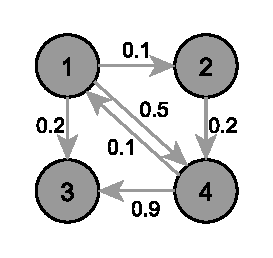
\includegraphics[width=0.37\linewidth]{images/ic.pdf}}
  \subfloat[\small{WC}\label{fig:wc}]{%
        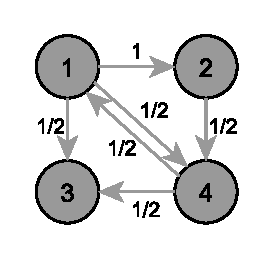
\includegraphics[width=0.37\linewidth]{images/wc.pdf}}
    \\% IMAGES HERE
  \caption{\small{\protect\subref{fig:ic} 
The directed graph $G = (V, E)$ for IC with independent diffusion probabilities. 
\protect\subref{fig:wc}
The directed graph for WC is obtained by setting the diffusion probabilities of incoming edges to $1 / |\Gamma^-_G(v)|$ for each vertex $v \in V$.% \kktodo{bu (4,1) kenarinin agirligi 1 degil mi?}\ggx{done.} 
  }}
  %\label{fig_ic_model} 
  \label{fig:xx} 
\end{figure}

\begin{itemize}[leftmargin=*]
\item The {\bf Independent Cascade} model works in rounds and activates a vertex $v$ in the current round if one of $v$'s incoming edges $(u, v)$ is 
used during the diffusion round, which happens with the activation probability $w_{u, v}$, given that $u$ has already been influenced in the previous rounds. The activation probabilities are independent (from each other and previous activations) in the {\em independent cascade} model which we concentrate on this paper. A toy graph with activation probabilities on the edges is shown in Figure~\ref{fig:ic}.
In theory, there can exist parallel and independent $\{u, v\}$ edges in $E$. In practice, they are merged to a single $\{u,v\}$ edge via preprocessing. 

\item The {\bf Weighted Cascade}  model is a variant of the independent cascade that uses the structural properties of vertices to set the edge weights as shown in Figure~\ref{fig:wc}.
The method, as described in~\cite{kempe2003maximizing}, sets $w_{u, v} = 1 / d_v$ where $d_v$ is the number 
of incoming edges of $v$~(which in the original graph is equal to $\Gamma^-_G(v)$).
Therefore, if $v$ has $\ell$ neighbors activated in the last round, its probability of activation in the new round is $1-( 1-1 / d_v)^\ell$. 
%\kktodo{bu tanim [7]'dekine uymuyor. Orada undirected graph var }\ggx{fixed.} 
% Note that the model is originally defined for undirected graphs in~\cite{kempe2003maximizing}. However, the definition above is consistent since one can consider each~(undirected) edge as two directed edges. 

%$ {|E^G_{u,v}|}/{|E^G_{u}|}$ where $|E^G_{u,v}|$ is the number of parallel $\{u, v\}$ edges and $|E^G_{u}|$ is the number of $\{u, .\}$ edges, i.e., all of $u$'s edges in the undirected graph.

\item{\bf Linear threshold} generalizes the independent cascade model and activates the vertex $v$ once the cumulative activation coming from its neighbors exceeds a given threshold $\theta_v$. 
All the $(u, v)$ edges with active $u$ vertices are taken into account in the process. Vertex $v$ is activated when the total activation probability through these edges exceeds $\theta_v$~\cite{kempe2003maximizing}.  
Therefore, the independent cascade model is a special variant of the LT model with $\theta_v = 0$. 
\end{itemize}

%As a generalization of the above-mentioned models, {\bf triggering} has also been proposed by Kempe~et~al.~\cite{kempe2003maximizing}. In this model, each neighbor has a probability to influence the vertex $v$. The diffusion process chooses a random subset of vertices called the {\em triggering set} to activate the vertices at each instance.
The complexity analysis stays consistent for many diffusion models, including {\em Independent Cascade}, {\em Weighted Cascade}, and {\em Linear Threshold} models; the time complexity of the greedy algorithm, estimating the $\sigma$ influence score, running $R$ simulations, and selecting $K$ seed vertices is $\mathcal{O}(KRn\sigma)$ for a graph with $n$ vertices. 
We concentrate on the IC model in this paper, but although their adaptation requires some work, the proposed methods are also relevant to other models in the literature.

\subsection{Count-Distinct Sketches}\label{sec:sketch}
The {\em distinct element count} problem focuses on finding the number of distinct elements in a stream where the elements are coming from a universal set ${\cal U}$. Finding the number of vertices to be influenced of a candidate seed vertex $u$, i.e., the cardinality of $u$'s {\em reachability set}, is a similar problem. For each sample subgraph, the number of visited vertices is found while traversing the subgraphs starting from $u$. Note that an exact computation of set cardinality requires memory proportional to the cardinality, which is ${\mathcal O}(|{\cal U}|)$. 

The reachability set of a vertex is the union of all its connected vertices (via outgoing edges). Many IM kernels exploit this property to some degree. The methods based on {\em reverse reachability} \cite{borgs2014maximizing} %\kktodo{cite}\ggx{done.} 
%and {\em bottom-up traversal} \\kktodo{cite} \ggx{buna referans dusunmem gerekli}
utilize this property directly to merge the reachability sets of connected vertices to estimate the number of vertices influenced. {\em MixGreedy} \cite{MixGreedy} %\kktodo{cite}\ggx{cited.} 
goes one step further; it utilizes the fact that for an undirected graph, all vertices in a connected component have the same reachability set. Therefore, all the reachability sets within a single sample subgraph can be found via a single graph traversal. 

For directed graphs, storing reachability sets for all vertices and merging these sets are infeasible for nontrivial graphs. 
If one-hot vectors are used to store the reachability sets for constant insertion time, $\mathcal{O}(n^2\mathcal{R})$ bits of memory is required where each merge operation has $\mathcal{O}(n)$ time complexity. 
If disjoints sets are used for storing reachability sets; $\mathcal{O}(n{\sigma}\mathcal{R})$ 
%\kktodo{Gokhan bunu aciklayalim, bir de $\bar{\sigma}$ nedir}\ggx{estimated influence} 
memory is required to store all reachability sets, and each merge operation has $\mathcal{O}({\tt Ack}(\sigma))$ complexity where ${\tt Ack}$ is the Ackermann~\cite{ackermann} function. %\kktodo{bu Ackermann'a atif verelim}.\ggx{done.}

Count-Distinct Sketches can be leveraged to estimate reachability sets' cardinality efficiently; for instance, the Flajolet–Martin~(FM) sketch~\cite{flajolet1985probabilistic} can do this with a constant number, $J$, of registers. Furthermore, the union of two sketches can be computed in constant time. The FM sketch stores that how rare the elements are in a stream. The rarity of the elements is estimated by counting the maximum number of leading zeros in the stream elements' hash values. Initially, each register is initialized with zero. The items are hashed one by one, and the length of the longest all-zero prefix is stored in the register. With a single register, the cardinality estimation can be done by computing the power $2^\ell$ where $\ell$ is the value in the register.

In practice, multiple registers and hash values, $M[j]$ and $h_j$, are commonly used to reduce variance. For a sketch with multiple registers, the impact of adding an item $x \in \cal{U}$ is shown in~\eqref{eq:sketch-add}:
\begin{equation}
    \label{eq:sketch-add}
    M[j] = \max(M[j], clz(h_j(x)),~1 \leq j \leq J
\end{equation} where $clz(y)$ returns the number of leading zeros in $y$ and $J$ is the number of sketch registers. With multiple registers, the average of the register values can be used to estimate the cardinality, and the result is divided to a correction factor $\phi \approx 0.77351$ to fix the error due to hash collisions. That is the estimated cardinality $e$ is computed as
\begin{equation}
    \label{eq:sketch-estimate}
    e = 2^{\bar{M}}/\phi
\end{equation} 
where $\bar{M} = {\tt{avg}}_j\{M[j]\}$ is the mean of the register values.

In this work, we utilize a variant of Flajolet–Martin sketch; since multiple Monte-Carlo simulations are performed to calculate the estimated influence, we use one register per simulation and take the average length of the longest leading zeros. Two given FM sketches $M_u$ and $M_v$ can be merged, i.e., their union $M_{uv}$ can be computed by taking the pairwise maximums of their registers. Formally; 
\begin{equation}
\label{eq:sketch-merge}
    M_{uv}[j] = \max(M_u[j], M_v[j]),~1 \leq j \leq J.
\end{equation} 
In our implementation, the merge operations are performed if and only if there is an edge between the vertices in respective samples. %\kktodo{burada simulations yaziyordu, anlamadim, iki simulation arasinda nasil edge olur - o yuzden vertex yazdim}. \ggx{ j'th sampleda vertexler arasında sampled edge olmasını kastetmiştim. Yanlis olmus.}  

\section{Efficient and Error-Adaptive Influence Maximization}\label{sec:method}

Most IM algorithms have the same few steps to find the best seed vertex set; sampling, building the influence oracle, verifying the impact of new candidates, and removing the latent seed set's residual reachability set. Following the idea proposed in~\cite{infuser}, \acro fuses the sampling step with other steps to avoid reading the graph multiple times. 

\acro first performs a diffusion process; the process starts with per-vertex sketches that are initialized with the hash value of the corresponding vertex~(i.e., every vertex reaches to itself). Then, for all the (sampled) edges ($u, v$), i.e., the ones that contribute to the diffusion for this simulation, the sketch of the source vertex $u$ is merged into that of the target vertex $v$ until all sketch registers for all the vertices converge. The merge operation utilized in this process is slightly different from the conventional one and retrofitted to mimic the IC diffusion. 

Throughout the process, each register is used only for a single sample/simulation. 
For an edge ($u, v$) in simulation $j$ where $v$ is a live vertex, an update, i.e., a merge operation, on $u$'s register is performed on the corresponding register $M_u$[$j$], i.e., $M_u[j] = max(M_u[j],M_v[j])$.
%if and only if the edge exists in the sample and \kktodo{bunu da degistirdim}\ggx{biz bunu yapmiyoruz, ben burada kayboldum.} $u$ is {\em live} in the current iteration. 
%A merge operation between sketch $M_u$,$M_v$ of vertices $u$,$v$,is only performed on $j$th register if there is a live edge between $u,v$ in sample $j$.
That is, at each iteration, vertices (outgoing) neighbors' reachability sets are added to their sketches.
This recursive formulation of the influence iteratively relays the reachability information among the vertices, allowing us to estimate the marginal influence for all vertices very fast.
%At each iteration, the sketches of the existing reachable vertices are modified. \kktodo{onceki cumleyi de degistirdim - dogru mu} \ggx{her vertex başkasına reachable olabilir, son cumleyi çıkartabilirz}
%Instead of simulating the diffusion sample-by-sample, vertex-by-vertex, or path-by-path, all the influence that passes through the edges in a single step is processed together. 

After estimating the reachability set cardinalities, \acro picks the vertex $v$ with the largest cardinality by evaluating the sketches. Then it finds the (actual) reachability set of the latent seed set, which is the union of the reachability sets of $v$ and the vertices in the seed set, by performing Monte-Carlo simulations. The vertices in this reachability set are removed from the live set $L$. %labeled as {\em visited}. 
%\kktodo{niye blocked, influenced desek?}\ggx{literaturde kullanilan terim o sekilde, ben visited'i tercih ederdim, algorithmaya gore live set L den çıkartıyoruz diye güncelledim.} 
Hence, in later iterations, these vertices will not contribute to the marginal gain. Finally, the algorithm checks if rebuilding is necessary for the sketches based on the difference between the sketch estimate and Monte-Carlo estimate. %\kktodo{yukaridaki cumlelerde bunlara isim verelim, burada soyleyelim matematiksel olarak - zaten isimleri var sanirim}.\ggx{malesef sembolleri,isimleri yok. $u \notin R_S$ şeklinde.} 

\subsection{Hash-based Fused Sampling}
The probabilistic nature of cascade models requires sampling subgraphs from $G = (V, E)$ to simulate the diffusion process. If performed individually as a preprocessing step, as the literature traditionally does, sampling can be an expensive stage, furthermore, a time-wise dominating one for the overall IM kernel. We identify two main bottlenecks; first, sampling multiple sub-graphs may demand multiple passes on the graph, which can be very large and expensive to stream to the computational cores, and second, if samples are memoized, the memory requirement can be a multiple of the graph size. 
In this work, we borrow the fused-sampling technique from {\sc InFuseR}~\cite{infuser} which eliminates the necessity of creation and storage of the sample subgraphs in memory. 
In Fig.~\ref{fig:traversal}, we briefly illustrate fused-sampling; instead of processing the samples independently as in Fig.~\ref{fig:sims}, fused-sampling processes each edge concurrently for multiple simulations as shown in Fig.~\ref{fig:fused}. This allows us to process each edge only a few times instead of once for every simulation.


\begin{figure}[!ht] 
    \centering
    %\subfloat[\label{fig:toy}]{%
    %   \includegraphics[width=0.47\linewidth]{sims-a%}}%  \\
    \subfloat[\label{fig:sims}]{%
        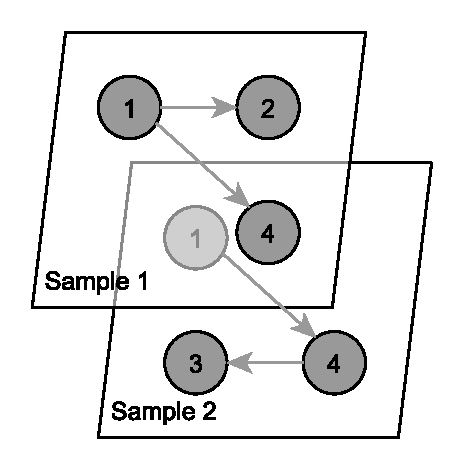
\includegraphics[width=0.5\linewidth]{images/samples.pdf}
    } 
    \subfloat[\label{fig:fused}]{%
     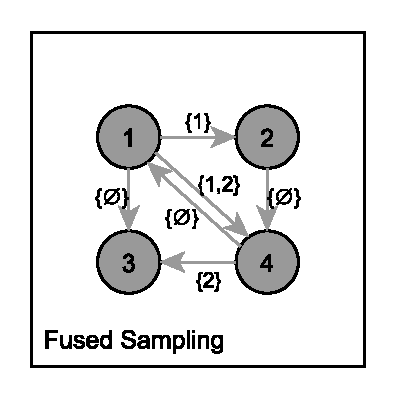
\includegraphics[width=0.5\linewidth]{images/fused.pdf}}
  \caption{\small{
  %\protect\subref{fig:toy} The toy graph 
  \protect\subref{fig:sims} Two sampled subgraphs of the toy graph from Figure~\ref{fig:ic} with 4 vertices and 6 edges.
  \protect\subref{fig:fused} The simulations performed are fused with sampling. Each edge is labeled with the corresponding sample/simulation IDs. 
  }}
  \label{fig:traversal} 
\end{figure}

In \acro, when an edge of the original graph is being processed, it is processed for all possible samples. Then, it is decided to be {\it sampled} or {\it skipped} depending on the outcome of the hash-based random value for each sample. Given a graph $G = (V, E)$, for an edge $(u, v) \in E$, the hash function used is given below:
\begin{equation}
    \label{eq:hash}
    h(u,v) = \mbox{{\sc Murmur3}}(u||v)~mod~2^{31}  
\end{equation}
where $||$ is the concatenation operator. In our preliminary experiments, we have tried a set of hash algorithms. After a careful analysis, we chose {{\sc Murmur3}} due to its simplicity and good avalanche behavior with a maximum bias $0.5\%$~\cite{MurmurHash3Performance}. Although the approach as mentioned above generates a unique hash value for each edge, and hence a unique sampling probability, different simulations require different probabilities. First, a set of uniformly randomly chosen numbers $X_r \in_R [0, h_{max}]$ associated with each simulation $r$ are generated to enable this for each edge. Then the sampling probability of $(u, v)$ for simulation $r$, $P(u, v)_r$, is computed: To do this, the hash value, $h(u,v)$, is XOR'ed with  $X_r$ and the result is normalized by dividing the value to the upper limit of the hash value $h_{max}$. Formally,
\begin{equation}
    \label{eq:hash_prob}
    P(u,v)_r = \frac{X_r \oplus h(u,v)}{h_{max}}.
\end{equation}
% The edge $\{u,v\}$ is verified to be in the sample if ${\rho}(u,v)_r$ is smaller than or equal to the threshold $w_{u,v}$. 
The edge $(u,v)$ exists in the sample $r$ if and only if  ${P}(u,v)_r$ is smaller than the edge threshold $w_{u,v}$. One of this approach's benefits is that an edge can be sampled using a single XOR and compare-greater-than operation. Moreover, the corresponding control flow branch overhead can be removed using {\em conditional move} instructions. 



\begin{figure}[!ht] 
    \centering
    \includegraphics[width=1\linewidth]{./images/CDF.pdf}
    \caption{\small{Cumulative probability function of hash-based sampling probabilities on various real-life networks.}}
    \label{fig:prob-cdf} 
\end{figure}


Using a strong hash function such as {{\sc Murmur3}} ensures that all bits independently change if the input is changed. This property allows us to generate good enough pseudo-random values for fair sampling. To evaluate the randomness and fairness of the values generated with the hash-based approach, we generated a large number of samples for various real-life networks and plotted the cumulative distribution~(Fig.~\ref{fig:prob-cdf}) and the bias of the random values $P(u,v)_r$ used~(Fig.~\ref{fig:prob-bias}). As the former shows, the sampling distribution of the hash-based computation values resembles a uniform random distribution. Furthermore, the latter shows that the bias is insignificant for each network. 

\begin{figure}[!ht] 
    \centering
    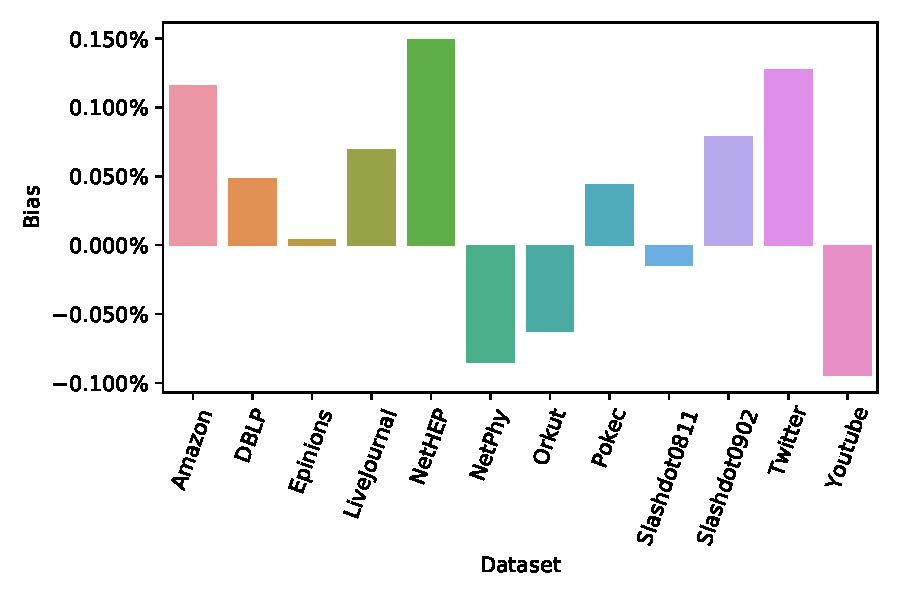
\includegraphics[width=1\linewidth]{./images/bias.pdf}
    \caption{\small{Bias distribution of hash-based sampling probabilities on various real-life networks.}}
    \label{fig:prob-bias} 
\end{figure}

% For a given graph $G = (V,E)$, the bias of a sampling probability $x$ is computed as $|(31/2) − E(|H(m)|) / E(|H(m)|))|$ for all $(u,v) \in E$ and $0 \leq r < R$. 
% Figure~\ref{fig:prob-bias} shows the bias for 12 real-life networks. 
%Traditional implementations sample each edge in $G$ once per simulation and store them to construct a sampled subgraph. n
Being able to generate the samples on the fly allows us to avoid many memory accesses. The only downside of hash-based fused sampling is that we have to generate all these random values,   $P(u,v)_r$, for each edge traversal and each simulation $r$. The edges' hash values are precomputed for all the edges in $E$ to reduce computation cost and leverage fused sampling's performance gains. Fortunately, the rest of the operations, i.e., one XOR and one division, are very fast on modern computing hardware. %The trade-off between extra memory and computation here maybe not be applicable for different computation architectures and faster/simpler hash functions.

\subsection{Estimating Reachability Set Cardinality}
A greedy solution to the influence maximization problem requires finding a vertex that maximizes the marginal influence gain at each step until the seed set size reaches $K$. For an exact computation, one must find all candidate vertices' reachability sets within all the samples. Such a task involves many graph traversals and is expensive even with various algorithmic optimizations and a scalable parallelized implementation, e.g., see~\cite{infuser}. The influence estimation problem is quite similar to the Count-Distinct problem applied to all sample subgraphs as explained above. Hence, in this work, we pursue the idea of using Count-Distinct sketches to estimate marginal influence scores. In this work, we propose an efficient and effective IM kernel, \acro, that utilizes Flajolet–Martin sketches described in Section~\ref{sec:sketch} to estimate the averages of distinct elements in the sampled subgraphs. Algorithm~\ref{algo:main} shows the steps taken by the kernel.


\begin{algorithm}
\caption{\sc{\acro}($G,K,J$)}
\label{algo:main}
\algorithmicrequire{$G = (V,E)$: the influence graph
\\\hspace*{6.6ex}{$K$: number of seed vertices
\\\hspace*{6.7ex}$J$: number of Monte-Carlo simulations}\\}
\algorithmicensure{$S$: a seed set that maximizes the influence on $G$
}
\begin{algorithmic}[1]
    \State {$S \leftarrow \{\emptyset\}$}
    \For{$ v\in V$} {\bf in parallel}
        \For{$ j\in J$}
            \State $M_v[j] \leftarrow clz(hash(v) \oplus hash(j))$ 
        \EndFor
    \EndFor
    \State $M \leftarrow ${\sc Simulate}$(G,M,J,\emptyset)$
    \State $M_{S'} \leftarrow zeros(J)$
    \State $\varsigma \leftarrow 0$
    \For{$k=1\ldots K$} \label{line:for}
        \State $s \leftarrow \underset{v\in V}{\mathrm{argmax}}\{${\sc Estimate}$(${\sc Merge}$(M_{S'},M_v))$\}\label{line:estimate}
        
        %\kktodo{S' nedir}\ggx{ latent seed set after rebuild}
        \State $S \leftarrow S \cup \{s\}$     
        \State $e \leftarrow ${\sc Estimate}$(${\sc Merge}$(M_{S'},M_s))$\label{line:e}
        % \State $R_S \leftarrow run\_cascade(G,S,J)$
        %\State {Compute $R_{G}(S)$; the reachability set of $S$}
        %\kktodo{buna da bir algoritma eklesek} }\ggx{Yayın konusu dışında kalabilir diye çıkartmıştık.}
        \State $R_G(S) \leftarrow$ reachability set of $S$ (for all simulations)
        \State $\sigma \leftarrow$ Monte-Carlo-based (actual) influence of $S$
        \State $\delta = \sigma - \varsigma$
        \State $err_l=|(e - \delta) / \delta|$
        \State $err_g=|(e-\delta) / \sigma|$
        \If{$ err_l < \epsilon_l \lor err_g < \epsilon_g$} %FIXME
            \State $M_{S'} \leftarrow$ {\sc Merge}$(M_{S'},M_s)$ \label{line:if}
        \Else 
            \For{$ v\in V$} {\bf in parallel}\label{line:else1}
                \For{$ j\in J$}
                    \State $M_v[j] \leftarrow clz(hash(v) \oplus hash(j))$ 
                \EndFor
            \EndFor
            \State $M \leftarrow ${\sc Simulate}$(G,M,J,R_{G}(S))$
            \State $M_{S'} \leftarrow zeros(J) $ 
            \State $\varsigma \leftarrow \sigma $ \label{line:else2} 
        \EndIf
    \EndFor
    \State \Return $S$
\end{algorithmic}
\end{algorithm}

 Algorithm~\ref{algo:main} first initializes the reachability sets of all vertices by adding the vertices themselves. 
 That is for all vertices $u$, its $j$th register is set to $M_u[j]=clz(h_j(u))$ meaning $R_{{G}_j}(u) = \{u\}$ where $G_j$ is the $j$th sampled graph. 
 Then, we perform the diffusion process on the sketch registers whose pseudocode is given in Algorithm~\ref{algo:diffusion-step}. The diffusion starts by adding all the vertices to the {\em live vertex set} $L$. 
 Then at each step, the incoming edges of the live vertices are processed. 
 For a vertex $u$, its sketch, $M_u$, is updated by merging the sketches $M_v$ of all live outgoing neighbors vertices $v \in {L} \cap \Gamma^+_{G}(u)$. For each such vertex $v$ and simulation $j$, the operation $M_u[j] = max(M_u[j], M_v[j])$ is performed. This approach can be seen as a bottom-up, i.e., reversed,  diffusion process where at each iteration, the cardinality information is pulled from vertices neighbors.
%  If a vertex $u$ is live, its outgoing edges $(u, v)$ s.t. $v \in \Gamma_G(v)$ are processed and the sketches of $v$ are merged into those of $u$. \kktodo{burada edgeleri tersten process ettigimizi aciklamamiz gerek} burasi yanlis
If any of $u$'s sketch registers changes during this operation it is added to the live vertex set $L'$ of the next iteration. Once the incoming edges of all live vertices are processed, the iteration ends. Figure~\ref{fig:hf-processing} shows how \acro performs two simulations at the same time using sketch registers.
 
 

\begin{algorithm}[!ht]
\caption{\sc{Simulate}($G,M,J,R_S$)}
\label{algo:diffusion-step}
\algorithmicrequire{$G = (V,E)$: the influence graph
\\\hspace*{6.6ex}{$M$: sketch vectors of vertices
\\\hspace*{6.7ex}${J}$: number of MC simulations
\\\hspace*{6.7ex}$R_S$: reachability set of the seed set
}
\\}
\algorithmicensure{$M$: updated Sketch vectors
}
\begin{algorithmic}[1]
    \State {$L \leftarrow V$}
    \State {$L' \leftarrow {\emptyset}$}
    \While{$|L|/|V| > \epsilon_c$}
        \For{$u \in \Gamma(L)$} {\bf in parallel} \label{ln:inner_start} %REVERSE THIS
        \For{$e_{u,v} \in A(u) $}
            \For{$j \in (0,J]$} \label{ln:vec1}
                \If{$P(u,v)_j < w_{u,v} \land u  \not\in R_S[j]$} \label{ln:early_exit}
                    \State{$M_u[j]\leftarrow max(M_u[j],M_v[j])$}\label{ln:update}          
                \EndIf
            \EndFor
            \If {$M_u$ changed}
                \State $L' \leftarrow L' \cup u $ \label{ln:inner_end}
            \EndIf
        \EndFor
        \EndFor
        \State $L \leftarrow L'$
        \State $L' \leftarrow \{\emptyset\}$
    \EndWhile
    \State \Return $M$
\end{algorithmic}
\end{algorithm}

 
\begin{figure*}[!ht]
    \begin{center}
    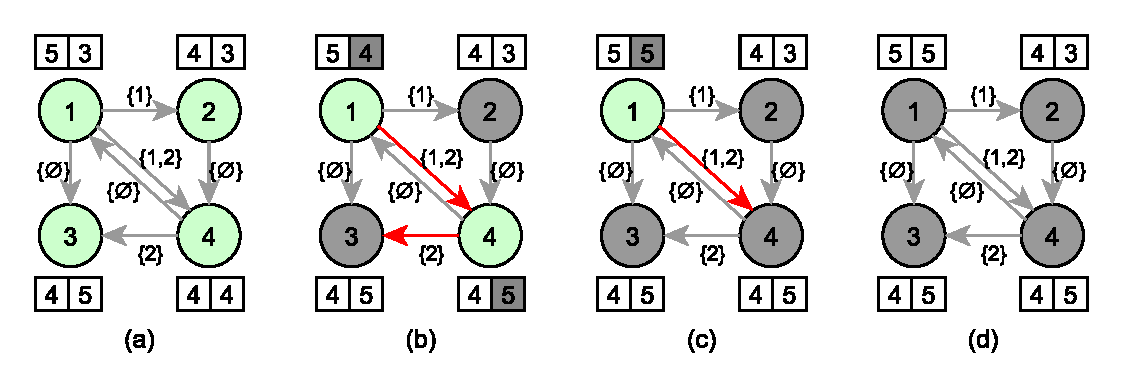
\includegraphics[width=0.7\linewidth]{images/sketch-diffusion.pdf}
    \caption{\small{(a) The initial state on the toy graph for \acro{}; all vertices are set as live~(green), and their registers are initialized with the length of the zero prefix of their hashes. (b) 
    % For all live edges,$e_{ij}$, respective registers are merged and set to source vertex $j$'s register, $M_j \leftarrow Max(M_i, M_j)$. 
    For the ($1, 4$) edge which is live for both simulations, 1's registers are set to the maximum of both 1's and 4's registers. The ($4, 3$) edge is live only in the second simulation. Hence, the second register of $4$ is updated to $5$. For the second iteration, vertices 1 and 4 are live~(green) since their registers have changed. (c) For the live ($1, 4$) edge, 1's second is updated and 1 is set as live again. (d) All the registers converged. As no live vertices exist, the process stops.}}\label{fig:hf-processing} 
    \end{center}
    \end{figure*} 
 
The traditional Greedy algorithm~\cite{kempe2003maximizing} processes the simulations one-by-one and computes the vertices' reachability sets. On the other hand, \acro efficiently performs multiple simulations at once in a single-step iteration. Since each iteration relays one level of cardinality information, this step requires at most $d$ iterations where $d$ is the diameter of $G$. When processed individually as the Greedy algorithm does, the $j$th simulation over the sampled subgraph $G_j$ would require only at most $d_j$ iterations, which is the diameter of $G_j$, and probably much smaller than $d$. Although \acro seems to perform much more iterations, $d$ is a loose upper bound for \acro. A better one is {\tt max}$\{d_j: 1 \leq j \leq J\}$ where $d_j$ is the diameter of $G_j$. To further reduce the overhead of concurrent simulations and avoid bottleneck simulations due to remaining perimeter vertices, we employ a early-exit threshold $\epsilon_c$ over the remaining live vertices ratio, which is expected to be very small when only one or two simulations remain. That is if $|L'| \leq |V| \times \epsilon_c$ the diffusion process in Algorithm~\ref{algo:diffusion-step} stops. Otherwise, $L$ is set to $L'$, $L'$ is cleared, and the next iteration starts. We used $\epsilon_c = 0.02$ to make \acro faster while keeping its quality almost the same.

After the diffusion process, the following steps are repeated until $K$ vertices are added to the seed set $S$. First, for each $v \in V$, the cardinality of the reachability set, $R_G(S \cup v)$, is estimated by merging $M_{S'}$ and $v$'s sketch registers where $M_{S'}$ is the set of sketch registers for the seed set $S$ used to estimate the number of already influenced vertices by $S$.\footnote{In fact, the definition is exact only if sketch rebuilding is disabled. As it will be described in the following subsection, when \acro's error-adaptive mechanism is enabled, $M_{S'}$ is periodically rebuilt to estimate the cardinality of reachability sets over the remaining, unblocked vertices. This is why $S'$ is used instead of $S$.} Before the kernel, these registers are initialized with zeros. Second, a vertex $s$ with the maximum cardinality estimation is selected and added to $S$. Third, the actual Monte-Carlo simulations are performed to compute the reachability set of the new seed set. Having an actual $R_G(S)$ allows us to calculate the estimation errors and find the blocked vertices for all simulations, which is vital since these blocked vertices can be skipped during the next diffusion steps. Besides, we leverage the actual influence score to have an {\em error-adaptive kernel}, i.e., to compute the actual sketch error and rebuild the sketches when the accumulated error reaches a critical level which can deteriorate the quality for the following seed vertex selections. 

\subsubsection{Error-adaptive sketch rebuilding}

Sketches are fast. However, each sketch operation, including update and merge, can decrease their estimation quality below a desired threshold. Our preliminary experiments revealed that sketches are highly competent at finding the first few seed vertices for influence maximization. Unfortunately, after a few seed vertices, the sketch registers $M_{S'}$, which are updated at line~\ref{line:if} of Algorithm~\ref{algo:main} via merging with new seed vertex $s$'s reachability set, become large. The saturation of $M_{S'}$ registers is important since \acro uses them to select the best seed candidate at line~\ref{line:estimate}. When they lose their sensitivity for seed selection, a significant drop in the quality is observed. 

\begin{figure}[!ht]
    \begin{center}
    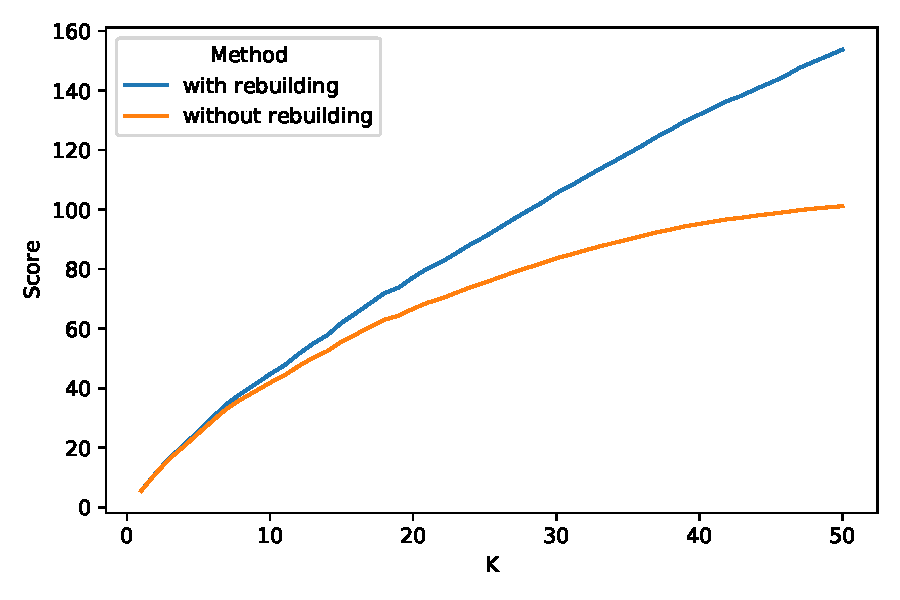
\includegraphics[width=\linewidth]{images/sketch-saturation.pdf}
    \caption{ Effect of register saturation on Amazon dataset using \acro($J=256$) without rebuilding against Greedy($\mathcal{R}=20000$) method\cite{kempe2003maximizing}. %\kktodo{buna TIMS'in sonuclarini da ekleyebilir miyiz - en kaliteli o diye, eger mavinin ustunde kaliyorsa guzel} \ggx{Bunun için süreye ihtiyacım var. Diğer algorithmlar mavi çizgi gibi olmalı,(SKIM hariç) 
     }\label{fig:sketch-saturation} 
    \end{center}
\end{figure}


\begin{figure*}[!ht]
    \begin{center}
        \subfloat[LiveJournal execution time in seconds\label{fig:lj-time}]{%
        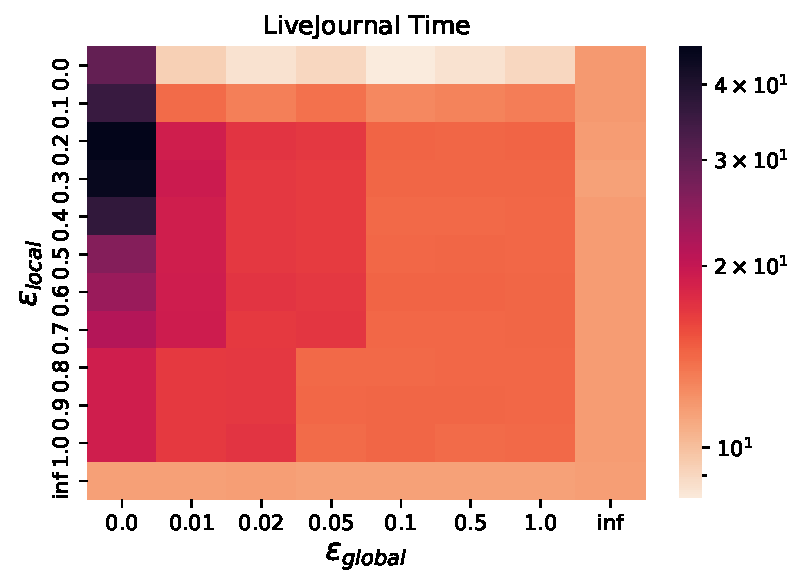
\includegraphics[width=0.33\linewidth]{images/heatmap_LiveJournal_time.pdf}
    }
    \subfloat[Orkut execution time in seconds\label{fig:orkut-time}]{%
        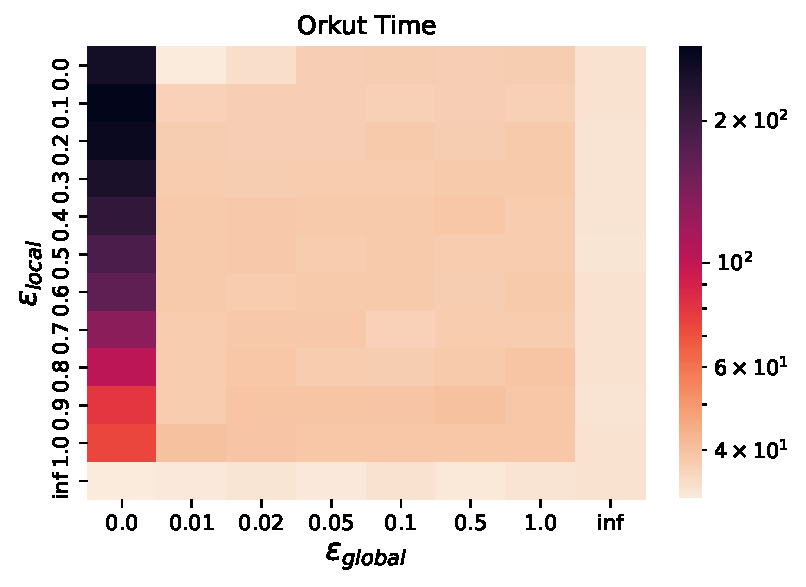
\includegraphics[width=0.33\linewidth]{images/heatmap_Orkut_time.pdf}
        }
    \subfloat[Pokec execution time in seconds\label{fig:pokec-time}]{%
        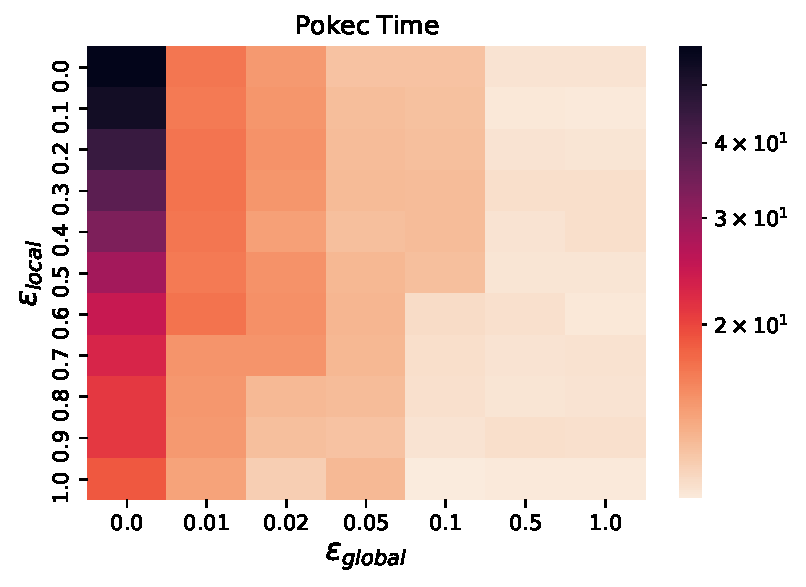
\includegraphics[width=0.33\linewidth]{images/heatmap_Pokec_time.pdf}
        }\\
        \subfloat[LiveJournal Influence Score\label{fig:lj-score}]{%
        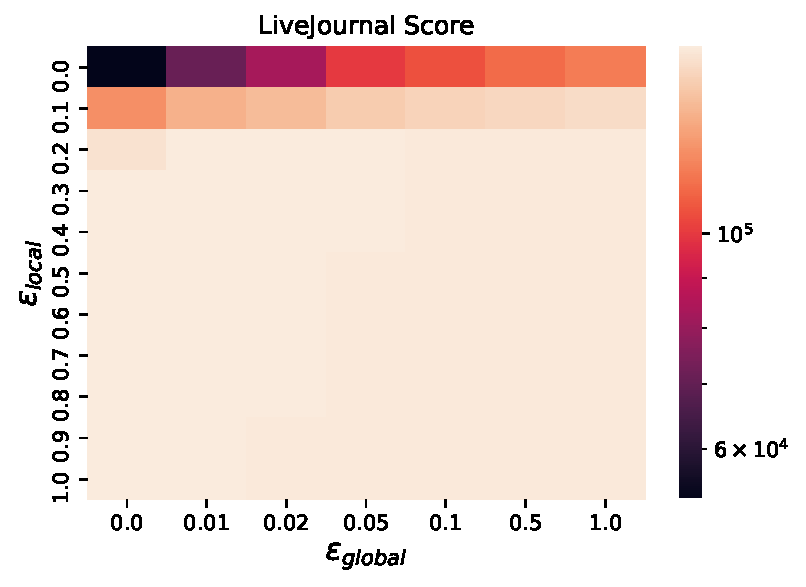
\includegraphics[width=0.33\linewidth]{images/heatmap_LiveJournal_score.pdf}
        }
    \subfloat[Orkut Influence Score\label{fig:orkut-score}]{%
        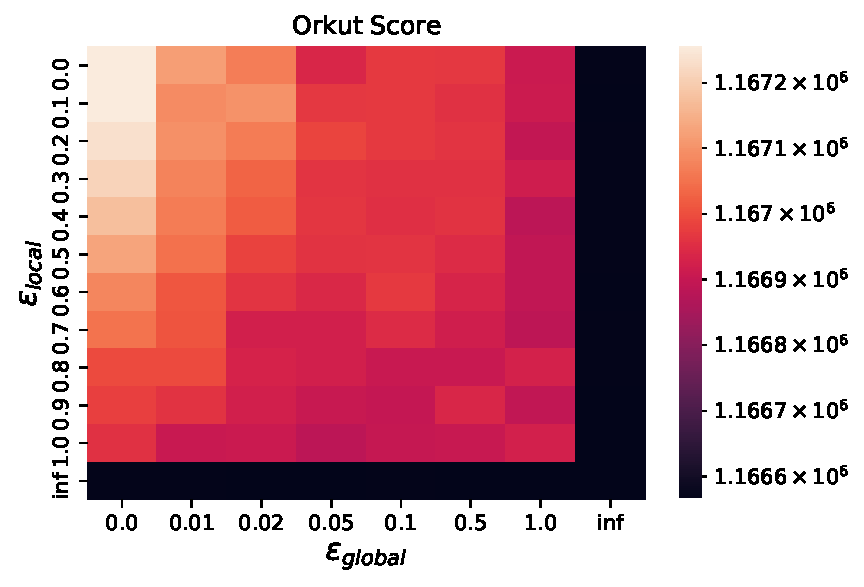
\includegraphics[width=0.33\linewidth]{images/heatmap_Orkut_score.pdf}
        }
    \subfloat[Pokec Influence Score\label{fig:pokec-score}]{%
        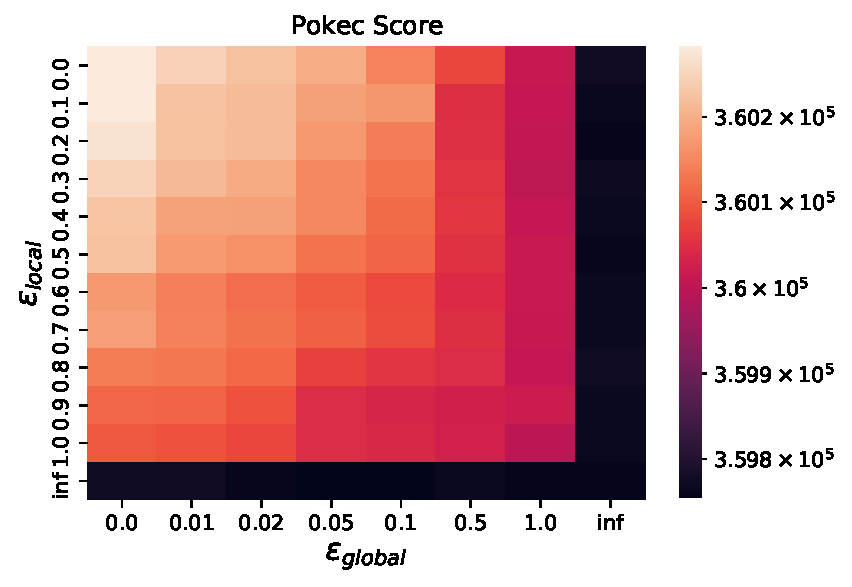
\includegraphics[width=0.33\linewidth]{images/heatmap_Pokec_score.pdf}
        }\\
    \end{center}
    \caption{Effect of $\epsilon$ parameters on \acro($J=256$, $\epsilon_c=0.02$) performance, using $\tau=18$ threads. Lighter shades are better. }\label{fig:parameter-smallmultiples} 
\end{figure*}    
%\begin{figure}[ht] 
%    \centering
%    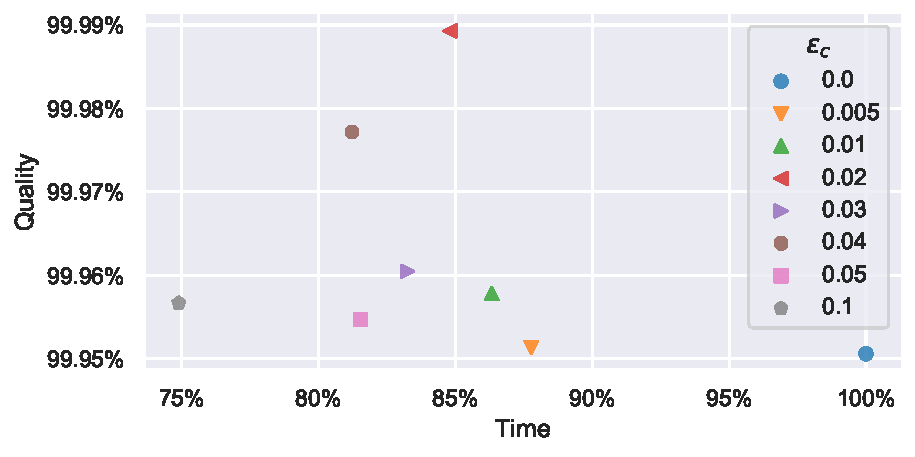
\includegraphics[width=1\linewidth]{images/converge-performance.pdf}
%  \centering \caption{Geometic mean of \acro's performance and results quality on different $\epsilon_c$ parameters ($J=256,\epsilon_l=0.3,\epsilon_g=0.01,\tau=18$) \kktodo{bu alttaki figurlerde sagdaki degerler sanki ters - kirmizi siyah bu sekilde mi siralanmali}. 
%    \label{fig:conv-perf}} 
%\end{figure}


Figure~\ref{fig:sketch-saturation} shows the effect of register saturation by comparing two \acro variants; the first one rebuilds a new sketch to choose each seed vertex $s$, i.e., the {\bf else} part in lines~\ref{line:else1}--\ref{line:else2} of Algorithm~\ref{algo:main} is executed for every iteration of the {\bf for} loop at line~\ref{line:for}. This sketch is built on the residual graph $G \setminus R_G(S)$, which remains after the current seed set's reachability is removed. The second variant builds a  sketch only once at the beginning and employs it through the IM kernel, i.e., the {\bf else} part is never executed. The figure shows that the latter's seed selection quality is comparable to that of the former for the first few seed vertices. However, a significant reduction in the quality is observed for the later vertices. Furthermore, the former approach's quality is on par with the expensive Greedy algorithm's quality, which computes actual reachability sets. This shows that sketch-based estimation can perform as well as the accurate but expensive approach. Note that rebuilding also allows \acro to work on a smaller problem for the following seed vertex selection since we remove the already influenced vertices from sample subgraphs and work on the remaining subgraphs. %Hence, for the remaining estimations, we only need to consider {\em latent} seed vertices of $S$ which are chosen after the sketch rebuild.

Although its quality is on par with the traditional algorithm, the variant which rebuilds a sketch for all the seed vertex selections can be expensive. Here, we leverage an error-adaptive approach by rebuilding them when a significant cardinality estimation error is observed. 
%As After adding vertices to the seed set, \acro performs Monte-Carlo simulations to estimate the reachability of the latent seed set.
The estimation error is calculated as follows; we store the influence score after each sketch rebuild in $\varsigma$~(line~\ref{line:else2} of Algorithm~\ref{algo:main}). Let $\sigma$ be the real influence for the seed set $S$ including the selected vertex. We first compute the marginal influence gain $\delta = \sigma - \varsigma$, which is the additional influence obtained since the last sketch rebuilt. Note that $e$, computed at line~\ref{line:e} is the sketch estimate for this value. \acro computes the local estimation error $err_l = |(e-\delta) / \delta|$ and the global error threshold $err_g=|(e-\delta) / \sigma|$. The sketches are assumed to be fresh if 
the local estimation error $err_l$ is smaller than a local threshold $\epsilon_{l}$ or the global error threshold $err_g=|(e-\delta) / \sigma|$ is smaller than a global threshold $\epsilon_{g}$.

%Before rebuilding stale sketches, the reachability set of the latent seed set, $R_G(S')$, is marked as visited and considered blocked in their respective simulations while rebuilding the sketches. Then, the sketches are rebuilt using Monte-Carlo simulations. After rebuilding, $M_{S'}$, which holds the seed vertices' cardinality estimate added after the last rebuild, is cleared with all zeros.
 
%This approach allows us to keep the sketches in high quality even after many vertices are added to the seed set. But on the other hand, it forces us to perform expensive Monte-Carlo simulations. 
%We reuse the reachability sets of the latent seed set, $R_G(S')$, computed by Monte-Carlo simulations. While rebuilding the sketches, $R_G(S')$ is used to check whether a vertex is blocked in a sample.

%Other methods mentioned in this paper do not report the time spent on calculating the influence scores, whereas our approach includes the time since it is crucial for keeping the sketches in high quality.

The use of two different, local and global, thresholds allows the algorithm to rebuild the sketches after significant local errors and skip this expensive process if the estimation error is insignificant compared to the total influence. As explained above, when the rebuilding is skipped, \acro only updates $M_{S'}$ by merging it with the candidate vertex's sketch. Hence, the selected threshold values, $\epsilon_{l}$ and $\epsilon_{g}$, have a significant impact on the performance. Setting $\epsilon_{l} = \epsilon_{g} = 0$ means that the algorithm always rebuilds. Conversely, setting $\epsilon_l = \epsilon_{g} = \infty$ will make \acro fast since sketches are built only once. However, the influence scores will suffer, which is already shown by Fig.~\ref{fig:sketch-saturation}. To evaluate the interplay and find the thresholds that yield a nice tradeoff, we conducted a grid search in which \acro's execution time and influence quality are measured for different parameters. The results of this preliminary experiment are shown in Figure~\ref{fig:parameter-smallmultiples}.  We found that the parameters $\epsilon_{l}=0.3$ and $\epsilon_{g}=0.01$ perform well on many datasets, both in terms of speed and quality. %For these experiments, $\epsilon_c = 0.02$ is used.


\subsection{Implementation Details}
%\subsection{Regularization and Vectorization}
%Sampled edges are stored together, diffusion related information stored afar. This way, SIMD operation is allowed on consecutively located edges, requiring random memory accesses for the diffusion process. Even if the sample or diffusion information are stored closely, without fusing, the random access overhead will be still there and much memory will be wasted. 

%One of the main advantages of fused sampling is allowing similar simulation data and computations together. For processing samples for an edge in algorithm \ref{algo:diffusion-step}~(lines~\ref{ln:inner_start}--\ref{ln:inner_end}).  

To efficiently process real-life graphs, \acro uses the Compressed Sparse Row~(CSR) graph data structure. In CSR, an array, $xadj$, holds the starting indices of the adjacency lists for each vertex, while another array, $adj$, holds the actual adjacency lists (i.e., the outgoing neighbors) one after another. Hence, the adjacency list of vertex $i$ is located in $adj$ at locations $adj[index[i], \ldots, index[i+1] - 1]$. 
    
The traditional two-step (sample-then-diffuse) computation model stores the (graph) data in a loosely coupled fashion.
% That is the data is clustered w.r.t. their simulation IDs. 
While designing \acro, we fine-tuned it to be vectorization friendly, including its data layout and computation patterns. These design choices allow us to perform multiple operations, i.e., the same operations but on different data, at once. For instance, we keep all the memory registers of a single vertex from different simulations adjacent, and this allows the efficient use of vectorized computation hardware while performing lines~\ref{ln:vec1}--\ref{ln:update} of Algorithm~\ref{algo:diffusion-step}. Also, random number generation, fused sampling, and sketch merging are vectorizable operations when the data are stored in a coupled way as in \acro.
%Vectorization also reduces branching on the overall computation; When vectorized, many comparison operations are done without branching. 

%We allow a single easy-to-predict branch after sample edges are generated to exit early without merging the registers. In our experiments, sorting random values $X_r$ significantly increases the performance by clustering similar simulations together. Since sorted random values are XOR'ed with the same edge hash values, it is more likely to non taken edges are sampled together. Up to 20\% speed-up can be achieved by an early exit at line \ref{ln:early_exit} using sorted random values.    
    
\section{Experimental Results}\label{sec:evaluation}
We performed the experiments on a server with an 18-core {\tt Intel Xeon Gold 6140}, running at 2.3Ghz, and 250GB memory. The Operating System on the server is {\tt Ubuntu 16.04 LTS} with 5.4.0-48 kernel. The algorithms are implemented using {\tt C++20}, and compiled with {\tt GCC 9.2.0} with {\tt "-Ofast"} and {\tt "-march=native"} optimization flags. Multi-thread parallelization was achieved with {\tt OpenMP} pragmas. {\tt AVX2} instructions are utilized by handcrafted code with vector intrinsics.

\begin{table}[!ht]
\caption{Properties of networks used in the experiments}\label{tab:NetProps}
\centering
\scalebox{0.95}{
\begin{tabular}{ll||r|r|r|r}
& & No. of           & No. of    & Avg.  &  Avg.  \\
&Dataset & Vertices          & Edges     &    Weight         &  Degree               \\
\hline
\multirow{6}{*}{\rotatebox[origin=c]{90}{Undirected}}& {\tt Amazon} & 262,113 & 1,234,878 & 1.00 & 4.71 \\
&{\tt DBLP} & 317,081 & 1,049,867 & 1.00 & 3.31 \\
&{\tt NetHEP} & 15,235 & 58,892 & 1.83 & 3.87 \\
&{\tt NetPhy} & 37,151 & 231,508 & 1.28 & 6.23 \\
&{\tt Orkut} & 3,072,441 & 117,185,083 & 1.00 & 38.14 \\
&{\tt Youtube} & 1,134,891 & 2,987,625 & 1.00 & 2.63 \\

\hline
\multirow{6}{*}{\rotatebox[origin=c]{90}{Directed}}&{\tt Epinions} & 75,880 & 508,838 & 1.00 & 6.71 \\
&{\tt LiveJournal} & 4,847,571 & 68,993,773 & 1.00 & 14.23 \\
&{\tt Pokec} & 1,632,803 & 30,622,564 & 1.00 & 18.75 \\
&{\tt Slashdot0811} & 77,360 & 905,468 & 1.00 & 11.70 \\
&{\tt Slashdot0902} & 82,168 & 948,464 & 1.00 & 11.54 \\
&{\tt Twitter} & 81,306 & 2,420,766 & 1.37 & 29.77 
\end{tabular}
}
\end{table}
\subsection{Experiment Settings}

We performed the experiments on twelve graphs~(six undirected, six directed). For comparability, graphs that have been frequently used within the Influence Maximization literature are selected. These graphs are {\tt Amazon} co-purchase network~\cite{snapnets}, {\tt DBLP} co-laboration network~\cite{snapnets}, {\tt Epinions} consumer review trust network, {\tt LiveJournal}~\cite{snapnets}, {\tt NetHEP} citation network~\cite{MixGreedy}, {\tt NetPhy} citation network~\cite{MixGreedy}, {\tt Orkut}~\cite{snapnets}, {\tt Pokec} Slovakian poker game site friend network~\cite{snapnets}, {\tt Slashdot} friend-foe networks~(08-11, 09-11)~\cite{snapnets}, {\tt Twitter} list co-occurence network~\cite{snapnets}, and {\tt Youtube} friendship network~\cite{snapnets}. The properties of these graphs are given in Table~\ref{tab:NetProps}. 

Three diffusion settings are simulated for a comprehensive experimental evaluation; for each network, we use 
\begin{enumerate}
    \item constant edge weights $w = 0.005$,
    \item constant edge weights $w = 0.01$~(as in~\cite{kempe2003maximizing} and~\cite{MixGreedy}),
    \item constant edge weights $w = 0.1$~(as in~\cite{kempe2003maximizing}),
    % \item weighted cascade edge weights $w_{u,v} = 1/|\Gamma(v)|$.
\end{enumerate}

We selected $w=0.005$ as a benchmark-setting to challenge \acro. Due to its diffusion algorithm's nature, \acro traverses vertices even if they are blocked, which happens faster when the graph is sparser. Also, for each live vertex, \acro processes the sample edges for all simulations. The other two settings are selected to emulate the experiments of~\cite{kempe2003maximizing} and~\cite{MixGreedy}.

\subsection{Performance Metrics}

The algorithms are evaluated based on (1) execution time, (2) influence score, and (2) maximum memory used. For Influence Maximization, there is a trade-off among these performance metrics; in one extreme, it is trivial to select random vertices as the seed set. In another, one can compute the reachability sets of every possible seed set of size $K$ and choose the best one. 
%The observed execution times and memory consumption of different algorithms are comparable when the algorithms run on the same computer.
In all our experiments, the execution times are the wall times reported by the programs. All the methods we benchmarked exclude the time spent on reading files and preprocessing. We only left out the time to spend on reading files for \acro. We allowed all methods to utilize all the CPU cores in all benchmarks, except {\sc Tim}, a single-threaded algorithm. The memory use reported in this paper is the {\em maximum resident set sizes}~(RSS), which are measured using GNU {\tt time} command.

Since the algorithms may use different methods to measure the influence score, the reported influence scores may not be suitable for comparison purposes with high precision. Due to this reason, we implemented an oracle with a straightforward, sample-then-diffuse algorithm without any optimization mentioned. For sampling, the random values are generated by the 32-bit Mersenne Twister pseudo-random generator {\tt mt19937} from {\tt C++} standard library. The same independent oracle obtains all influence scores in this paper.


\subsection{Algorithms evaluated in the experiments}

We evaluated our method against three other state-of-the-art influence maximization algorithms, {\sc Tim}, {\sc Skim}, and {\sc Imm}. The first algorithm focuses on the influence score, whereas the second is a sketch-based algorithm that takes the execution time into account. Last, the third one is an approximation algorithm with a parameter to control the approximation quality.
\begin{itemize}
\item The two-phased Influence Maximization~({\sc Tim}) consists of two phases: {\em Parameter Estimation} and {\em Node Selection}~\cite{tim}. The first phase computes a lower bound on the maximum expected influence to spread among all size-$K$ node sets and then uses it to derive a parameter $\theta$. The second phase randomly samples $\theta$ reverse reachability sets from $G$ and then derives a size-$K$ vertex-set $S$ that covers a large number of these sets.

\item The sketch-based Influence Maximization~({\sc Skim}) is a parallel algorithm which uses a combined bottom-$k$ min-hash reachability sketch~\cite{bottomk} with $k = 64$ to estimate the influence scores of the seed sets~\cite{cohen2014sketch}. {\sc Skim} employs $\ell = 64$ sampled subgraphs and designed and tuned to provide good seed sets in a short time. 

\item Minutoli et al.'s {\sc Imm} is a high-performance, parallel algorithm that efficiently produces accurate seed sets~\cite{minutoli2019fast}. 
It is an approximation method that improves the Reverse Influence Sampling~(RIS)~\cite{borgs2014maximizing} algorithm by eliminating the need for the threshold to be used. %{\sc Imm} generalizes the influence of all vertices on a small set of sample graphs that is sampled from the reachability sets of a few vertices. 
We have used $\epsilon = 0.5$ as suggested in the original paper, where $\epsilon$ is a user-defined parameter to control the approximation boundaries.
\end{itemize}
%Finally, our method \acro employs both Monte-Carlo simulations and count-distinct sketches for estimating reachability set cardinalities. Even though \acro is blazing-fast and accurate for limited $K$, we exploit the performance of the method to improve the results by rebuilding sketches after removing residual influence networks.

%%%%%%%%%%%%%%%%%%%%%%%%%%%%%%%%%%%%%%%%%%%%%%%%%%%%%%%%%%%%%%%%%%%%%


\begin{table*} %TABLE 5+7
    \caption{\acro execution times~(in secs), memory use~(in GBs), and influence scores on the networks with $K = 50$ seeds using $\tau=18$ threads and constant edge weights $w=0.005$. Influence scores are given relative to \acro{}. }
    \label{tab:timings005}
    \centering
    \scalebox{0.94}{
\begin{tabular}{l|rrrr|rrrr|rrrr}
\toprule
{} & \multicolumn{4}{c|}{Time} & \multicolumn{4}{c|}{Score} & \multicolumn{4}{c}{Memory} \\
Method & {\sc Hyper} &    {\sc Tim} &    {\sc Imm} &  {\sc Skim} & {\sc Hyper} &    {\sc Tim} &     {\sc Imm} &    {\sc Skim} & {\sc Hyper} &  {\sc Tim} &  {\sc Imm} & {\sc Skim} \\

Dataset      & {\sc Fuser} &         &         &         & {\sc Fuser} &         &         &         & {\sc Fuser} &       &       &      \\

\midrule
{\tt Amazon}       &       1.30 &  124.38 &   5.58 & 63.73 &       96.9 &  1.041x &  1.000x &  0.562x &       0.17 & 21.62 & 0.90 & 6.78 \\
{\tt DBLP}         &       1.61 &  177.99 &   5.71 & 28.24 &      106.6 &  1.068x &  1.027x &  1.036x &       0.27 & 31.24 & 0.95 & 3.12 \\
{\tt Epinions}     &       1.11 &   12.16 &   0.50 &  8.29 &      635.3 &  1.026x &  1.001x &  0.939x &       0.06 &  0.78 & 0.07 & 1.04 \\
{\tt LiveJournal}  &      13.25 & 4172.69 & 118.82 & 19.35 &    37174.1 &  1.010x &  0.995x &  0.957x &       3.97 & 27.43 & 2.78 & 2.00 \\
{\tt NetHEP}       &       0.31 &    2.22 &   0.31 &  1.96 &       80.2 &  1.065x &  0.993x &  0.871x &       0.01 &  0.80 & 0.04 & 0.33 \\
{\tt NetPhy}       &       0.39 &    7.40 &   0.40 &  1.00 &      124.5 &  1.042x &  0.999x &  0.777x &       0.03 &  2.01 & 0.08 & 0.16 \\
{\tt Orkut}        &      30.22 &       - & 780.22 & 41.82 &   158842.6 &       - &  0.997x &  1.001x &       5.19 &     - & 7.81 & 1.77 \\
{\tt Pokec}        &      11.05 &  149.34 &   5.04 & 18.40 &     1095.1 &  1.032x &  1.027x &  0.925x &       1.57 & 10.16 & 1.40 & 1.74 \\
{\tt Slashdot0811} &       1.18 &    6.93 &   0.40 &  1.00 &      576.4 &  1.015x &  0.983x &  0.942x &       0.06 &  0.76 & 0.09 & 0.13 \\
{\tt Slashdot0902} &       1.14 &    6.96 &   0.40 &  1.17 &      610.5 &  1.022x &  0.998x &  0.953x &       0.06 &  0.71 & 0.08 & 0.14 \\
{\tt Twitter}      &       1.10 &  171.17 &   5.40 &  1.60 &     3458.7 &  1.006x &  0.990x &  0.942x &       0.09 &  2.02 & 0.12 & 0.15 \\
{\tt Youtube}      &       1.95 &   46.61 &   2.42 & 13.24 &     1820.8 &  1.025x &  1.013x &  1.000x &       0.73 &  3.96 & 0.48 & 1.39 \\
\bottomrule
Norm. arit. mean &&69.39x&4.37x&8.13x&&1.032x&1.002x&0.909x& &42.60x&2.05x&9.76x \\ 
Norm. geo. mean &\multicolumn{1}{c}{all}&28.19x&1.69x&3.47x&\multicolumn{1}{c}{all}&1.032x&1.002x&0.899x&\multicolumn{1}{c}{all}&22.75x&1.65x&3.58x \\ 
Norm. max perf&\multicolumn{1}{c}{1.00x}&314.92x&25.82x&49.02x&\multicolumn{1}{c}{1.000x}&1.068x&1.027x&1.036x&\multicolumn{1}{c}{1.00x}&127.18x&5.29x&39.88x \\ 
Norm. min perf&&5.88x&0.34x&0.85x&&1.006x&0.983x&0.562x&&5.43x&0.66x&0.34x \\ 

\end{tabular}\\
    }
    \end{table*}
    
    \begin{table*} %TABLE 5+7
    \caption{\acro execution times~(in secs), memory use~(in GBs), and influence scores on the networks with $K = 50$ seeds using $\tau=18$ threads and constant edge weights $w=0.01$. Influence scores are given relative to \acro{}. }
    \label{tab:timings01}
    \centering
    \scalebox{0.92}{

% \begin{tabular}{lrrrrrrrrrrrr}
% \toprule
% {} & \multicolumn{4}{l}{Time} & \multicolumn{4}{l}{Score} & \multicolumn{4}{l}{Memory} \\
% Method & HyperFuser &    TIM &     IMM &   SKIM & HyperFuser &    TIM &     IMM &    SKIM & HyperFuser &  TIM &   IMM & SKIM \\
\begin{tabular}{l|rrrr|rrrr|rrrr}
\toprule
{} & \multicolumn{4}{c|}{Time} & \multicolumn{4}{c|}{Score} & \multicolumn{4}{c}{Memory} \\
Method & {\sc Hyper} &    {\sc Tim} &    {\sc Imm} &  {\sc Skim} & {\sc Hyper} &    {\sc Tim} &     {\sc Imm} &    {\sc Skim} & {\sc Hyper} &  {\sc Tim} &  {\sc Imm} & {\sc Skim} \\

Dataset      & {\sc Fuser} &         &         &         & {\sc Fuser} &         &         &         & {\sc Fuser} &       &       &      \\
\midrule
{\tt Amazon }       &       0.96 &  107.94 &    3.28 &  59.32 &      152.7 &  1.037x &  1.024x &  0.390x &       0.17 & 18.11 &  0.55 & 6.40 \\
{\tt DBLP }         &       0.73 &   73.37 &    2.85 &  18.71 &      233.5 &  1.043x &  1.005x &  0.997x &       0.27 & 11.92 &  0.52 & 2.05 \\
{\tt Epinions }     &       0.82 &  112.08 &    3.78 &   5.07 &     2480.1 &  1.006x &  0.983x &  0.984x &       0.06 &  1.95 &  0.10 & 0.68 \\
{\tt LiveJournal }  &      16.72 &       - &  386.37 &  16.23 &   155375.8 &       - &  0.996x &  0.993x &       3.97 &     - &  6.64 & 1.45 \\
{\tt NetHEP }       &       0.26 &    1.84 &    0.23 &   1.89 &      129.1 &  1.036x &  0.997x &  0.826x &       0.01 &  0.60 &  0.03 & 0.31 \\
{\tt NetPhy }       &       0.24 &    3.33 &    0.23 &   0.86 &      320.5 &  1.010x &  0.985x &  0.732x &       0.03 &  0.67 &  0.05 & 0.12 \\
{\tt Orkut }        &      42.37 &       - & 1870.35 & 114.82 &   650157.1 &       - &  1.000x &  1.000x &       5.19 &     - & 20.13 & 3.43 \\
{\tt Pokec }        &      11.65 & 4148.03 &   88.89 &   7.25 &    44685.8 &  1.004x &  0.996x &  0.988x &       1.57 & 39.98 &  2.09 & 0.78 \\
{\tt Slashdot0811 } &       0.84 &  102.96 &    3.70 &   0.87 &     2882.1 &  1.003x &  0.984x &  0.976x &       0.06 &  2.01 &  0.10 & 0.08 \\
{\tt Slashdot0902 } &       0.90 &  129.31 &    4.19 &   0.88 &     3061.5 &  1.008x &  0.992x &  0.980x &       0.06 &  2.42 &  0.11 & 0.08 \\
{\tt Twitter }      &       0.90 &  390.36 &   10.96 &   1.22 &     9628.6 &  1.004x &  0.992x &  0.978x &       0.09 &  4.91 &  0.23 & 0.09 \\
{\tt Youtube }      &       2.18 &  534.41 &   14.86 &  16.97 &     9042.7 &  1.009x &  0.994x &  1.006x &       0.73 &  7.10 &  0.48 & 1.73 \\
\bottomrule
Norm. arit. mean &&167.17x&9.73x&9.99x&&1.016x&0.996x&0.904& &42.91x&2.09x&8.26x \\ 
Norm. geo. mean &\multicolumn{1}{c}{all}&100.14x&5.45x&3.58x&\multicolumn{1}{c}{all}&1.016x&0.996x&0.879x&\multicolumn{1}{c}{all}&36.26x&1.91x&2.82x \\ 
Norm. max perf&\multicolumn{1}{c}{1.00x}&433.73x&44.14x&61.79x&\multicolumn{1}{c}{1.000x}&1.043x&1.024x&1.006x&\multicolumn{1}{c}{1.00x}&106.53x&3.88x&37.65x \\ 
Norm. min perf&&7.08x&0.89x&0.62x&&1.003x&0.983x&0.390x&&9.73x&0.66x&0.37x \\ 

% Geo. Mean wrt.&1.000x&100.140x&5.448x&3.582x&1.000x&1.016x&0.996x&0.879x&1.000x&36.264x&1.909x&2.820x \\ \acro
\end{tabular}



    }
    \end{table*}
    \begin{table*} %TABLE 5+7
    \caption{\acro execution times~(in secs), memory use~(in GBs), and influence scores on the networks with $K = 50$ seeds using $\tau=18$ threads and constant edge weights $w=0.1$. Influence scores are given relative to \acro{}. }
    \label{tab:timings1}
    \centering
    \scalebox{0.92}{

\begin{tabular}{l|rrrr|rrrr|rrrr}
\toprule
{} & \multicolumn{4}{c|}{Time} & \multicolumn{4}{c|}{Score} & \multicolumn{4}{c}{Memory} \\
Method & {\sc Hyper} &    {\sc Tim} &    {\sc Imm} &  {\sc Skim} & {\sc Hyper} &    {\sc Tim} &     {\sc Imm} &    {\sc Skim} & {\sc Hyper} &  {\sc Tim} &  {\sc Imm} & {\sc Skim} \\

Dataset      & {\sc Fuser} &         &         &         & {\sc Fuser} &         &         &         & {\sc Fuser} &       &       &      \\
\midrule
{\tt Amazon}       &       0.69 &  133.22 &    1.98 &  23.62 &    11797.0 &  1.006x &  0.990x &  0.815x &       0.17 &   5.49 &  0.23 & 2.59 \\
{\tt DBLP }         &       0.54 & 1368.83 &   14.54 &   6.30 &    48549.9 &  1.001x &  0.995x &  1.001x &       0.27 &  35.19 &  1.06 & 0.65 \\
{\tt Epinions }     &       0.26 &  439.33 &    5.46 &   9.42 &    18409.9 &  1.000x &  0.998x &  0.997x &       0.06 &  12.17 &  0.39 & 1.18 \\
{\tt LiveJournal }  &      10.10 &       - & 1071.30 &  65.73 &  2134726.0 &       - &  1.000x &  1.000x &       3.97 &      - & 65.49 & 1.40 \\
{\tt NetHEP }       &       0.10 &   14.18 &    0.33 &   0.61 &     2461.7 &  1.002x &  0.975x &  0.899x &       0.01 &   1.02 &  0.04 & 0.10 \\
{\tt NetPhy }       &       0.16 &  107.52 &    1.53 &   0.34 &     8339.5 &  1.007x &  0.994x &  0.975x &       0.03 &   3.84 &  0.13 & 0.03 \\
{\tt Orkut }        &      16.55 &       - & 1964.83 & 446.92 &  2692366.5 &       - &  1.000x &  1.000x &       5.19 &      - & 71.94 & 9.68 \\
{\tt Pokec }        &       4.90 &       - &  514.79 &  31.80 &  1034859.8 &       - &  1.000x &  1.000x &       1.57 &      - & 26.46 & 0.98 \\
{\tt Slashdot0811 } &       0.21 &  677.49 &    7.34 &   2.44 &    25871.8 &  1.000x &  1.000x &  0.999x &       0.06 &  19.10 &  0.59 & 0.25 \\
{\tt Slashdot0902 } &       0.23 &  695.12 &    7.99 &   2.35 &    27519.5 &  1.000x &  1.000x &  0.999x &       0.06 &  18.45 &  0.66 & 0.24 \\
{\tt Twitter }      &       0.33 & 1897.50 &   16.09 &   1.62 &    55327.3 &  1.000x &  0.998x &  0.998x &       0.09 &  34.56 &  1.04 & 0.05 \\
{\tt Youtube }      &       1.12 & 7158.56 &   60.59 &  30.57 &   171392.9 &  1.000x &  0.999x &  1.001x &       0.73 & 139.12 &  4.19 & 2.88 \\
\bottomrule
Norm. arit. mean &&2624.61x&47.17x&15.37x&&1.002x&0.996x&0.974x& &199.54x&8.79x&5.32x \\ 
Norm. geo. mean &\multicolumn{1}{c}{all}&1449.41x&27.87x&11.06x&\multicolumn{1}{c}{all}&1.002x&0.996x&0.972x&\multicolumn{1}{c}{all}&163.77x&7.15x&2.63x \\ 
Norm. max perf&\multicolumn{1}{c}{1.00x}&6391.57x&118.72x&36.23x&\multicolumn{1}{c}{1.000x}&1.007x&1.000x&1.001x&\multicolumn{1}{c}{1.00x}&384.00x&16.85x&19.67x \\ 
Norm. min perf&&141.80x&2.87x&2.13x&&1.000x&0.975x&0.815x&&32.29x&1.35x&0.35x \\ 
\end{tabular}


    }
    \end{table*}
    
 \begin{figure}[!ht] 
     \centering
     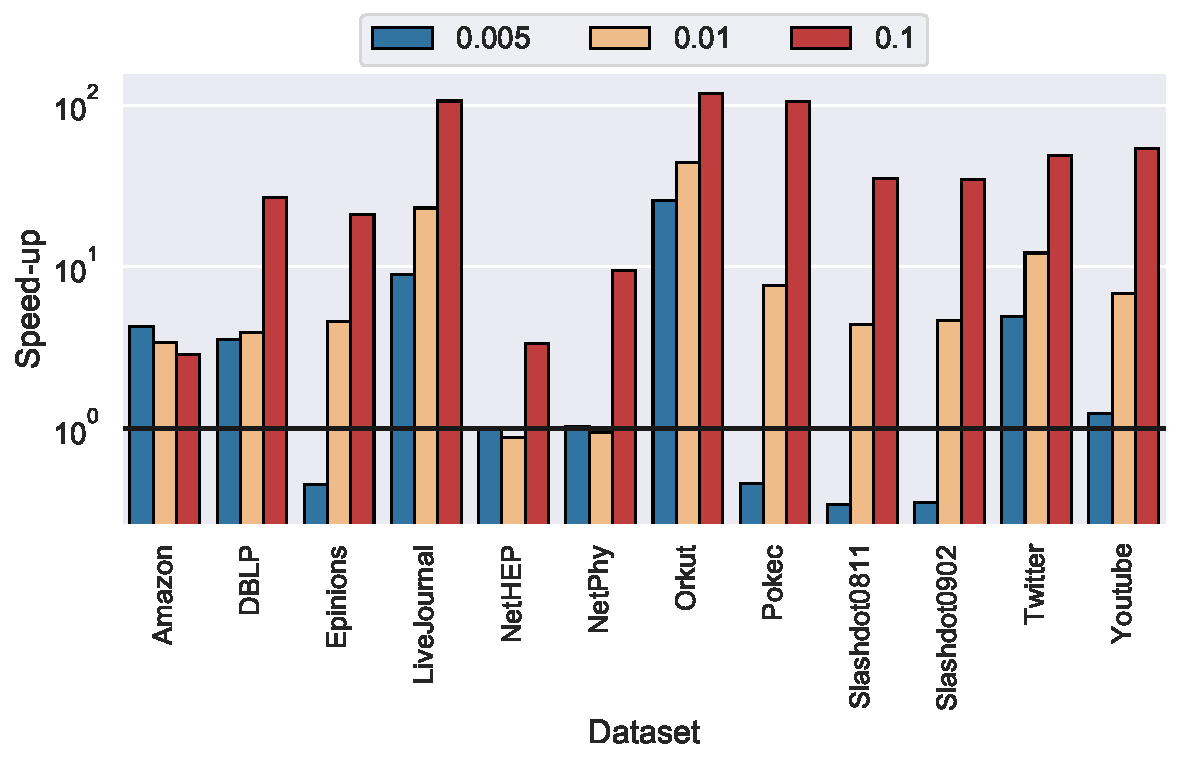
\includegraphics[width=1\linewidth]{images/speedup-imm}
   \centering \caption{Speed-up obtained by \acro{} over {\sc Imm}($\epsilon\myeq 0.5$) using $\tau=18$ threads.
     \label{fig:vs-imm}} 
 \end{figure}

 \begin{figure}[!ht] 
     \centering
     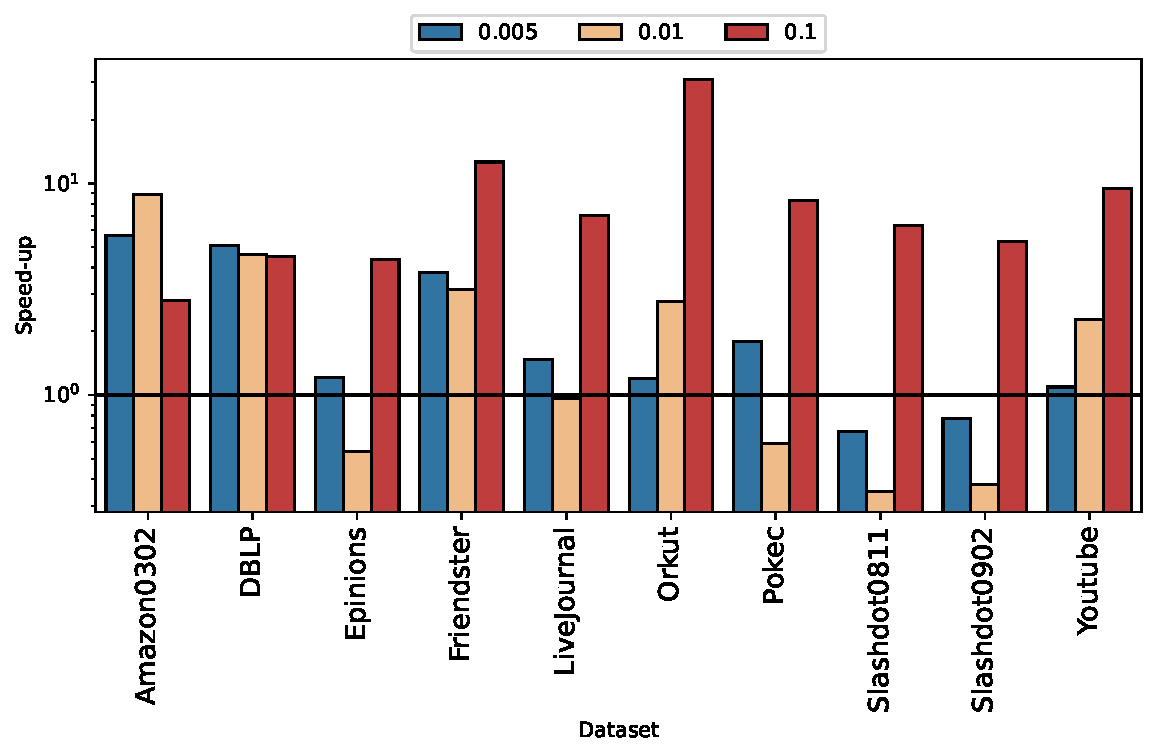
\includegraphics[width=1\linewidth]{images/speedup-skim}
   \centering \caption{Speed-up obtained by \acro{}($J=256$) over {\sc Skim}($r\myeq 64,l\myeq 64$) using $\tau=18$ threads.
     \label{fig:vs-skim}} 
 \end{figure}

\subsection{Comparing \acro with State-of-art}
To compare the run time, memory use, and quality of \acro with those of the state-of-the-art, %As explained above, the parameters of the experimented methods are hard to compare directly. It is infeasible to find precisely the corresponding parameter between any two methods in this setting. For that reason, we have used the parameters suggested by the paper.
we perform experiments using the parameters suggested by the authors of these tools: {\sc Tim} ($\epsilon=0.3$), {\sc Imm} ($\epsilon=0.5$), {\sc Skim} ($l=64,k=64$). 
In short, these parameters are controlling the quality of the seed sets. In fact, one of the drawbacks of \acro is that it does not have a direct control over the approximation factor, whereas {\sc Tim} and {\sc Imm} have one. Still, \acro can control the quality indirectly by tuning the number of Monte-Carlo simulations $J$ which also increases the number of sketches used per vertex. In the experiments, we set $J = 256$, which is comparable in quality to other methods. As explained in the previous section, we use global error threshold as $\epsilon_{g} = 0.01$, local error threshold as $\epsilon_l=0.3$, and the early-exit ratio as $\epsilon_{c}=0.02$. 

Compared to \acro, for $w = 0.005$~(Table~\ref{tab:timings005}), i.e., sparser samples, \acro is 

For small graphs such as {\tt NetHep}, {\tt NetPhy}, and {\tt Amazon}, the results show that {\sc Tim} has $4\%$--$7\%$ more influence score, whereas the sketch-based algorithm {\sc Skim} has $13\%$--$44\%$ less influence. While \acro is having a hard time catching edges in samples; \acro has a chance of capturing an edge is $1-(1-0.005)^{256}=0.72$, {\sc Tim} will not suffer from the situation but {\sc Skim}  suffer much worse capturing vertices in sketches. On the performance side, \acro is superior to other methods, Amazon dataset only takes 1.3 seconds, including Monte-Carlo influence oracle computations. {\sc Skim} and {\sc Imm} take 63.73 and 124.38 seconds. For 4\% quality improvements, {\sc Imm} is $\sim$100 slower than \acro. For small improvements in quality, we can always double the number of registers/simulations $J=256$ to $512$, which would approximately double the wall time. For the same $w=0.005$ and larger graphs such as {\tt LiveJournal} and {\tt Orkut}, the quality gap narrows {\sc Skim}  only $5\%$ behind, and {\sc Tim} is marginally better. 

The performance gap also narrows between \acro and {\sc Skim}, \acro only $30\%$ faster in small $w$. In the same setting, {\sc Tim}  takes 1.5 hours for {\tt LiveJournal}, could not finish {\tt Orkut}; crashing after consuming all memory available. 
For $w=0.1$, \acro is much faster than all other methods and still provides high-quality results. While all methods are struggling with problem size, \acro converge results much faster, even faster than previous experiment settings. Also, the memory consumption stays the same for all experimental settings, much smaller than other methods.

Performance characteristics of \acro are very different from its state-of-the-art competitors. \acro's performance depends on the influence graph's diameter, whereas other methods mentioned in this paper depend on the influence score. Due to this reason, we observe highly varying performance speed-up results in tables \ref{tab:timings005}-\ref{tab:timings1}. In exceptional settings, such as the Pokec dataset and $w=0.01$ where the influence network's diameter is around 43, \acro loses its edge against its fastest competitor. On the other hand, in the same dataset with $w=0.1$, the diameter is only around 17; \acro is six times faster than its nearest competitor. Running time of \acro decreases as connections gets stronger and influence graph gets denser, whereas other methods gets slower.

When we compare \acro's performance to {\sc Imm} in figure \ref{fig:vs-imm}, we can see that \acro is almost always faster except few settings. The setting $w=0.005$ is especially challenging for \acro due to the high diameter of the influence graph and low vector unit utilization. Except for the {\tt Pokec} dataset, all the other experiments \acro performs worse takes slightly longer than 1 second. In such a small time scale and small influence, \acro is suffering death by thousand cuts. Only a few hundreds of vertices can be activated, whereas we optimize \acro to work on much larger scale problems. For the {\tt Pokec} dataset, \acro performs many graph traversals for minimal gains and spends twice as much time, 11 seconds, yet still beating other competitors. For a small price of influence,\acro could have performed much faster, but in our experiments, we aimed for high-quality results. 

In figure \ref{fig:vs-skim}, we compared \acro's performance with {\sc Skim}. \acro performs much better, both in terms of quality and speed, in near all settings. For the notorious {\tt Pokec} dataset \acro performs better then {\sc Skim}, except for $w=0.01$; the diameter of influence graph does not affect {\sc Skim}'s performance. {\sc Skim} performs slightly better in terms of speed in that setting but it has worse result quality. In some settings such as {\tt Amazon}($w=0.01$), {\sc Skim} performed very poorly; only 39\% of the influence was achieved with respect to \acro, and {\sc Skim} spent 59.32 seconds where as \acro could finish in 0.96 seconds.


Memory consumption of \acro is linearly dependent on the number of vertices in the graph. Both sketch-registers and visited information are stored per vertex so that \acro's memory consumption stays constant for any simulation parameters or any number of edges. In all benchmark settings, \acro consumed significantly less memory on average. The competitors' memory usage behavior differs between parameters and datasets; \acro's memory use is predictable for any graph, \acro consumes only $O(R)$ bytes per vertex.%12*R bits aslinda 

\subsection{Scalability with multi-threaded parallelism}

\begin{figure*}[!ht] 
    \centering
    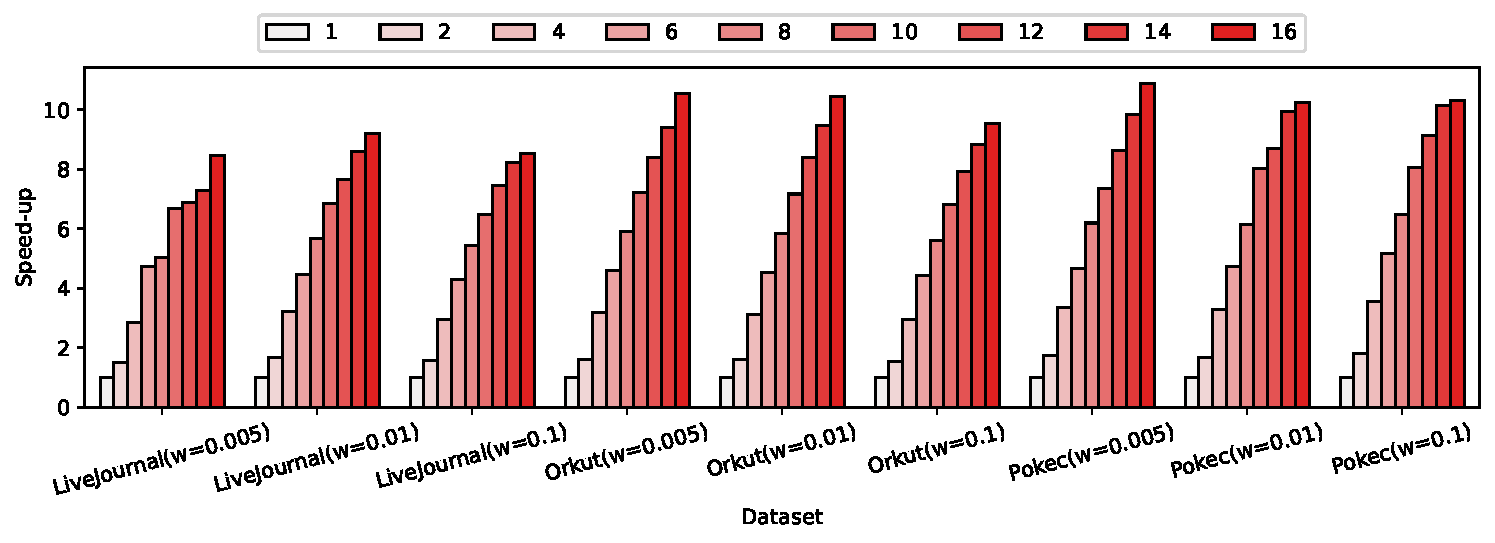
\includegraphics[width=\linewidth]{images/threads.pdf}
   \centering \caption{Scaling of \acro with multiple threads on some of largest datasets in the benchmarks.
     \label{fig:scaling}} 
\end{figure*}

In our implementation, we used a {\em pull-based} approach in which the vertices~(processed at line~\ref{ln:inner_start} of Algorithm~\ref{algo:diffusion-step}) pull the influence, i.e., reachability set cardinality estimations, from their outgoing neighbors. A classical {\em push-based} approach, in which the vertices relay their influence to their outgoing neighbors could also be leveraged. However, the push-based approach makes a (target) vertex register potentially updated at the same time in different computation units. Specifically, the update operation~(corresponding to the one at line~\ref{ln:update} of Algorithm~\ref{algo:diffusion-step}) of the {\em pull-based} approach will be the cause of race conditions. One can easily argue that since we are already using sketches, and not computing exact cardinalities, such race conditions are acceptable and they will not reduce the quality of influence estimations. However, the performance may suffer due to false sharing. Figure~\ref{fig:scaling} shows \acro's speedup values obtained via a simple {\tt OpenMP} parallelization at line~\ref{ln:inner_start} of Algorithm~\ref{algo:diffusion-step}. Even though the pull-based diffusion shows a nice parallel performance, it is possible to implement \acro using other approaches such as the {\em queue-based} approach which may improve performance by only processing live vertices. The pull-based diffusion method is chosen due to its simplicity and scalability to many threads/compute units.

\section{Related Work}\label{sec:relatedwork}

Although they can be inferior in terms of influence, modern IM algorithms are shown to be quite fast compared to conventional simulation-based approaches such as {\sc MixGreedy}. Techniques such as using GPUs~\cite{IMGPU,curipples}, sketches for finding set intersections~\cite{cohen2014sketch,IPA}, reverse sampling to estimate influence from a small subset of vertices\cite{borgs2014maximizing,minutoli2019fast}, and estimating the necessary number of simulations/samples required for each step greatly reduces asymptotic boundaries of execution time~\cite{leskovec2009community}.

\acro borrows much from {\sc InFuseR}~\cite{infuser}, including hash-based fused sampling. {\sc InFuseR} computes influence by memoizing connected components for all vertices and only can work on {\em undirected} datasets. It also employs CELF optimization to reduce cardinality computations. On the other hand, \acro can process both directed and undirected graphs and uses the Flajolet–Martin sketches in a novel way to estimate cardinality and choose seed candidates. 

Sketch-based IM methods are cheaper compared to simulation-based methods. They usually pre-compute the sketches by processing the graph for evaluating the influence spread instead of running simulations repetitively. One of the popular methods for sketch-based influence maximization is {\sc Skim}~\cite{cohen2014sketch} by Cohen~et~al. {\sc Skim} is a parallel algorithm which uses combined bottom-$k$ min-hash reachability sketches~\cite{bottomk,cohen2015all} with $k = 64$, and $\ell$ sampled subgraphs, to estimate the influence scores of the seed sets~\cite{cohen2014sketch}. In this work, we preferred Flajolet-Martin~\cite{flajolet1985probabilistic} sketches instead for their simplicity, suitability for vectorization and fused sampling, and hence, execution-time performance. 

The Independent Path Algorithm~(IPA)~\cite{IPA} by Kim~et~al. runs a proxy model and prunes paths with probabilities smaller than a given threshold in parallel. The approach only keeps a dense but small part of the network and scalable to only sparse networks. Liu~et~al. proposed IMGPU~\cite{IMGPU}, an IM estimation method by utilizing a bottom-up traversal algorithm. It performs a single Monte-Carlo simulation on many GPU threads to find the reachability of the seed set. It is $5.1\times$ faster than {\sc MixGreedy} on a CPU. The GPU implementation is up to $60\times$ faster with an average speed-up of  $24.8\times$. 

Borgs~et~al.~\cite{borgs2014maximizing} proposed Reverse Influence Sampling~(RIS), which samples a fraction of all random reverse reachable sets. The number of necessary samples to find the seed set with $K$ vertices is calculated based on the number of visited vertices. The algorithm has an approximation guarantee of $(1-1/e-\epsilon)$. Minutoli et al. improved RIS and proposed {\sc Imm} that works on multi-threaded and distributed architectures~\cite{minutoli2019fast} with high efficiency. Recently, the authors extended the algorithm to work in a multi-GPU setting~\cite{curipples}.

Two-phased Influence Maximization~({\sc Tim}) borrows ideas from RIS but overcomes its limitations with a novel algorithm design~\cite{tim}. The first phase computes a lower bound of the maximum expected to spread among all size-$k$ node sets. It then uses the lower bound to derive a parameter $\theta$. In the second phase, it samples $\theta$ random RR sets from $G$, and then derives a size-k node-set $\hat{S}$ that covers a large number of RR sets.

%Cohen~\cite{cohen2015all} presented the Historic Inverse Probability ({\sc HIP}) estimators which, when applied to All-Distance Sketches, outperforms the {\sc HyperLogLog} sketches~\cite{flajolet2007hyperloglog} while estimating the number of distinct elements on data streams. In this work, we preferred Flajolet-Martin~\cite{flajolet1985probabilistic} instead of bottom-$k$ min-hash sketches for simplicity and execution-time performance. In future work, other estimators such as HIP can be used to improve \acro.


Kumar and Calders~\cite{kumar2017information} proposed the Time Constrained Information Cascade Model and an IM kernel that works on the model using versioned HyperLogLog sketches. The algorithm computes the influence for all vertices in an interaction graph while performing a single pass over the data. The sketches are used for each time window to estimate active edges. On the other hand, \acro uses $J$ sketches for each vertex to estimate the marginal influence and employs a rebuilding strategy for fast processing. \acro also utilizes fused sampling and error adaptive rebuilding of sketches.

\section{Conclusion and Future Work}\label{sec:conclusion}

In this work, we propose a sketch-based Influence Maximization algorithm that employs fused sampling and error-adaptive rebuilding. We provide a fast implementation of the algorithm that utilizes multi-threading to exploit multiple cores. Also, we present a performance comparison with state-of-the-art IM algorithms on real-world datasets. 
With the proposed method, \acro can achieve $\maxspeedupSKIM\times$ speed-up against a sketch-based algorithm {\sc Skim} and $\maxspeedupIMM\times$ speed-up against an approximation-based algorithm {\sc Imm} while producing high-quality seed sets. 

In the future, we will extend our work to a distributed GPGPU setting to process graphs with billions of vertices and edges. The main issue with \acro on such an architecture is the broadcast of sketch registers. When the vertices are partitioned into different computation units, resulting sketch updates should be communicated to all partitions. To overcome the issue and reduce communication bottlenecks, graph preprocessing and speculative diffusion strategies will be employed.


%%%%%%%%%%%%%%%%%%%%%%%%%%%%%%%%%%%%%%%%%%


\ifCLASSOPTIONcaptionsoff
  \newpage
\fi

\bibliographystyle{IEEEtran}
\bibliography{refs}
\begin{IEEEbiography}[{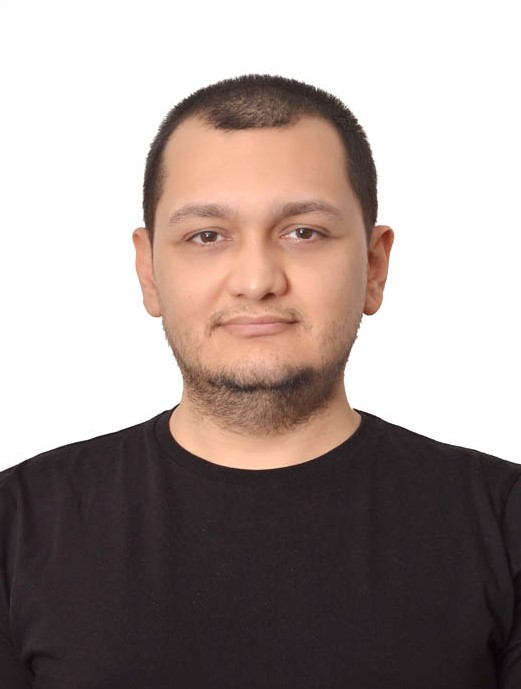
\includegraphics[width=1in,height=1.25in,clip,keepaspectratio]{./images/gokhan.png}}]{G\"{o}khan~G\"{o}kt\"{u}rk} is a PhD candidate at the Faculty of Engineering and Natural Sciences in Sabancı University. He has received his BS and MS degrees from Sabancı University as well. He is interested in High Performance Computing, Parallel Programming, and Graph Processing.
\end{IEEEbiography}
\begin{IEEEbiography}[{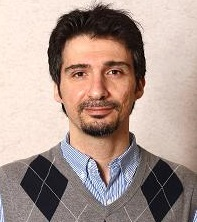
\includegraphics[width=1in,height=1.25in,clip,keepaspectratio]{./images/kamer.jpg}}]{Kamer Kaya} is an Asst. Professor at Sabancı University. After receiving his PhD from Bilkent University, he worked at CERFACS, France, as a post-graduate researcher in the Parallel Algorithms Project. He then joined the Ohio State University in September 2011 as a postdoctoral researcher, and in December 2013, he became a Research Assistant Professor in the Dept. of Biomedical Informatics.
His current research interests include Parallel Programming, High-Performance Computing, and Cryptography. 
\end{IEEEbiography}

\end{document}


